% -*- TeX-PDF-mode: t -*-
% rubber: rules rules.ini

\documentclass[letterpaper,twocolumn,10pt]{article}

\newif\ifdraft\draftfalse
\newif\ifnotes\notesfalse
\newif\ifinternal\internalfalse

\ifdraft\else\notesfalse\internalfalse\fi

%\usepackage[letterpaper,body={6.5in,9in}]{geometry}
\usepackage{usenix,endnotes}
\usepackage{mathptmx}
\usepackage{ptmgreek}
\usepackage{amsmath}
\usepackage{amssymb}
\usepackage{framed}
\usepackage{color}
\usepackage{xspace}
\usepackage{graphicx}
\usepackage{ifthen}
%<bug avoidance from http://www.about-here.org/about_here/2007/08/latex-using-els.html>
\makeatletter
\newif\if@restonecol
\makeatother
\let\algorithm\relax
\let\endalgorithm\relax 
%</bug avoidance>
%\usepackage{algorithm2e}
\usepackage[ruled,vlined]{algorithm2e}
\usepackage{nicefrac}
\usepackage{url}
\usepackage{cite}
\usepackage[margin=-25pt,format=hang,listofformat=subparens]{subfig}
\IfFileExists{microtype.sty}{
  \usepackage[stretch=10,shrink=10]{microtype}
%  \usepackage{microtype}
}{
  \PackageError{microtype}{Package microtype not found.  Please
    install texlive-latex-recommended}{}
}
\ifdraft
\usepackage{hginfo}
\fi

\ifdraft
\fancyfoot[L]{{\bf \ifinternal{\small{VMware INTERNAL CONFIDENTIAL}} \fi DRAFT}}
\fi

% Disable page numbers in final copy
\ifdraft\else\pagestyle{empty}\fi

% Avoid widows and orphans
\widowpenalty=500
\clubpenalty=500

% http://www.tug.org/mail-archives/pdftex/2007-December/007480.html
% This screws up blending, but at least doesn't throw us into CMYK if
% there is any alpha
\pdfpageattr {/Group << /S /Transparency /I true /CS /DeviceRGB>>}

\newcommand{\DeDe}{{\sc{DeDe}}\xspace}
\newcommand{\SHORTCUT}{{\sc{shortcut}}\xspace}

\newboolean{includeShortcut}
\setboolean{includeShortcut}{false}
%\setboolean{includeShortcut}{true}
\newcommand{\incShortcut}[1]
{
  \ifthenelse{\boolean{includeShortcut}}
             {{#1}\xspace}{\vspace{0in}}
}

\definecolor{shadecolor}{rgb}{0.9,0.9,0.9}
\ifnotes
\newenvironment{notes}[1][]{\begin{shaded}}{\end{shaded}}
\else
\newenvironment{notes}[1][]{\PackageError{main}{Notes environment found}}
\fi

\long\def\internal#1{
  \ifinternal
  \begin{shaded}
    \leavevmode % Avoid a bug in shaded at the top of a page
    #1
  \end{shaded}
  \else\fi
}

\def\urltilda{\lower .7ex\hbox{\~{}}\kern .04em}

\def\ie{{\it i.e.}}
\def\eg{{\it e.g.}}

\def\shaone{SHA\nobreakdash-1\xspace}

% -*- TeX-master: "paper.tex"; TeX-PDF-mode: t -*-

% some useful macros

% Tuple typesetting
% Adds triangle brackets and spaces commas.  ie $\tup{1,2,3}$
% Arguments can be enclosed in braces or angle brackets
\makeatletter
\def\tup{%
  \def\tupInside\tupStart##1,##2\tupEnd{%
    ##1
    \def\tempa{}\def\tempb{##2}
    \ifx\tempa\tempb\else
    ,\;\tupInside\tupStart##2\tupEnd
    \fi}
  \def\tupBraces##1{\left\langle\tupInside\tupStart##1,\tupEnd\right\rangle}
  \def\tupBrackets<##1>{\tupBraces{##1}}
  \@ifnextchar<\tupBrackets\tupBraces}
\makeatother

\definecolor{xxxcolor}{rgb}{0.8,0,0}
\makeatletter
\long\def\XXX{\@ifnextchar[{\@XXX}{\@XXX[]}}
\long\def\@XXX[#1]{\@ifnextchar[{\@@@XXX{#1}}{\@@XXX{#1}}}
\ifnotes
% Show XXX comments
\long\def\@@XXX#1{{\color{xxxcolor} XXX #1\xspace}}
\long\def\@@@XXX#1[#2]{{\color{xxxcolor} XXX (#1) #2\xspace}}
\else
% Hide XXX comments
\long\def\@@XXX#1{\ignorespaces}
\long\def\@@@XXX#1[#2]{\ignorespaces}
\fi
\makeatother


\begin{document}

% -*- TeX-master: "paper.tex"; TeX-PDF-mode: t -*-

\title{Decentralized~Deduplication in SAN~Cluster~File~Systems}
% Decentralized Deduplication in SAN Cluster~File~Systems and Hypervisors
% Decentralized Deduplication in a [Shared Disk] Virtual Environment?
% Decentralized Deduplication for SAN Cluster~File~Systems

% Conjoined email addresses
% \author{Austin T. Clements$^*$ $\qquad$
%   Irfan Ahmad $\qquad$
%   Murali Vilayannur $\qquad$
%   Jinyuan Li \\
%   \small{\sf aclements@csail.mit.edu} $\qquad$
%   \small{\sf $\{$irfan,muraliv,jli$\}$@vmware.com} \\
%   \small{VMware, Inc.} $\qquad$ \small{$^*$MIT}}

\iftrue

\author{
  \begin{tabular}[t]{c}
    {\rm Austin T. Clements}$^*$ %\\ \small{\sf aclements@csail.mit.edu}
    \and
    {\rm Irfan Ahmad} %\\ \small{\sf irfan@vmware.com}
    \and
    {\rm Murali Vilayannur} %\\ \small{\sf muraliv@vmware.com}
    \and
    {\rm Jinyuan Li} %\\ \small{\sf jli@vmware.com}
  \end{tabular} \\
  VMware, Inc. $\;$ $^*$MIT CSAIL}

\else

% This is a more literal interpretation of the template file on the
% USENIX site, but none of the papers in USENIX '08 listed any
% institution more than once, so I went with the deduplicated form
% above.

\author{
  {\rm Austin T. Clements}\\
  MIT CSAIL
  \and
  {\rm Irfan Ahmad}\\
  VMware, Inc.
  \and
  {\rm Murali Vilayannur}\\
  VMware, Inc.
  \and
  {\rm Jinyuan Li}\\
  VMware, Inc.
}

\fi

\date{}

% ACM SIG-style authors
% \numberofauthors{4}
% \author{
% \alignauthor
% Austin Clements\\
%     \affaddr{VMware Inc.}\\
%     \email{aclements@vmware.com}
% \alignauthor
% Irfan Ahmad\\
%     \affaddr{VMware Inc.}\\
%     \email{irfan@vmware.com}
% \alignauthor 
% Murali Villayannur\\
%     \affaddr{VMware Inc.}\\
%     \email{muraliv@vmware.com}
% \and
% \alignauthor
% Jinyan Li\\
%        \affaddr{VMware Inc.}\\
%        \email{jli@vmware.com}
% }
%\additionalauthors{Additional authors: someone else (email: {\texttt{xxx@vmware.com}}), someone else2 (email: {\texttt{yyy@vmware.com}}).}

\maketitle


\begin{abstract}
\input{abstract}
\end{abstract}

% -*- TeX-master: "paper.tex"; TeX-PDF-mode: t; ispell-local-pdict: "words" -*-

\section{Introduction}

Deployments of consolidated storage using Storage Area Networks (SANs)
are increasing, motivated by universal access to data from
anywhere, ease of backup, flexibility in provisioning, and centralized
administration.  SAN arrays already form the backbone of modern data
centers by providing consolidated data access for multiple hosts
simultaneously.  This trend is further fueled by the proliferation of
virtualization technologies, which rely on shared storage to support
features such as live migration of virtual machines (VMs) across hosts.

SANs provide multiple hosts with direct SCSI access to shared
storage volumes.  Regular file systems assume exclusive
access to the disk and would quickly
corrupt a shared disk.  To tackle this, numerous shared disk cluster
file systems have been developed, including VMware
VMFS~\cite{vmfsdatasheet}, RedHat GFS~\cite{preslan99gfs}, and IBM
GPFS~\cite{schmuck02gpfs}, which use distributed locking to coordinate
concurrent access
%to the shared file system
between multiple hosts.

Cluster file systems play an important role in virtualized data
centers, where multiple physical hosts each run potentially hundreds
of virtual machines whose virtual disks are stored as regular
files in the shared file system.  SANs provide hosts access to shared storage
for VM disks with near native SCSI performance while also enabling
advanced features like live migration, load balancing, and failover of
VMs across hosts.

These shared file systems represent an excellent opportunity for
detecting and coalescing duplicate data.  Since they store data from
multiple hosts, not only do they contain more data, but data
redundancy is also more likely.  Shared storage for VMs is a
ripe application for deduplication because common system
and application files are repeated across VM disk images and hosts can
automatically and transparently share data between and within VMs.
This is especially true of virtual desktop infrastructures
(VDI)~\cite{vdi-doc}, where desktop machines are virtualized,
consolidated into data centers, and accessed via thin clients.  Our
experiments show that a real enterprise VDI deployment can expend as much as
80\% of its overall storage footprint on duplicate data from VM disk
images. Given the desire to lower costs, such waste provides
motivation to reduce the storage needs of virtual machines both in
general and for VDI in particular.

Existing deduplication techniques~\cite{bolosky00sis, douceur02farsitededup, 
  hydrastor-fast09, centeradatasheet, hong04sandedup,
  netapp-asis-website, quinlan02venti, rhea-foundation,
  zhu08datadomain}
\XXX[Austin][Cut down the more redundant ones?]
rely on centralized file systems, require cross-host communication for
critical file system operations, perform
deduplication in-band, or use content-addressable storage.
All of these approaches have limitations in our domain.
Centralized techniques would be difficult to extend to a setting with
no centralized component other than the disk itself.  Existing
decentralized techniques require cross-host communication for most
operations, often including reads.  Performing
deduplication in-band with writes to a live file system can degrade
overall system bandwidth and increase IO latency.  Finally,
content-addressable storage, where
data is addressed by its content hash, also suffers from performance
issues related to expensive metadata lookups as well as loss of
spatial locality~\cite{cas-experiences}.

% Austin: Specifically, we need something decentralized both because
% our FS is decentralized and because we can't suffer the performance
% or fault tolerance impact of a centralized solution.  We can't do
% deduplication in-band because our file system is live and we can't
% cache the index in a decentralized setting.  CAS suffers from
% similar performance penalties in our setting and destroys spatial
% locality.

Our work addresses deduplication in the decentralized setting of
VMware's VMFS cluster file system.  Unlike existing solutions, \DeDe
coordinates a cluster of hosts to cooperatively perform block-level
deduplication of the live, shared file system.  It takes advantage of
the shared disk as the only centralized point in the system and does not
require cross-host communication for regular file system operations,
retaining the direct-access advantage of SAN file systems.  As a
result, the only failure that can stop deduplication is a failure of
the SAN itself, without which there is no file system to deduplicate.
Because \DeDe is an online system for primary storage, all
deduplication is best-effort and performed as a background process,
out-of-band from writes, in order to minimize impact on system
performance.  Finally, unlike other systems, \DeDe builds block-level
deduplication atop an existing file system and takes advantage of
regular file system abstractions, layout policy, and block addressing.
As a result, deduplication introduces no additional metadata IO when
reading blocks and permits in-place writes to blocks that have no
duplicates.

\XXX[Deduplication is completely transparent to virtual machines
running on top.]

% Finally, \DeDe is built atop an existing file system and
% takes advantage of regular file system abstractions, layout policy,
% and block addressing.  \XXX[And no impact on unique blocks]

% Unlike CAS, \DeDe uses content hashes only for the purpose of
% detecting duplicates.

This paper presents the design of \DeDe.  We have implemented a
functional prototype of \DeDe for VMware ESX Server~\cite{esx-doc}
atop VMware VMFS.  Using a variety of synthetic and realistic
workloads, including data from an active corporate VDI installation,
we demonstrate that \DeDe can reduce VM storage requirements by
upwards of 80\% at a modest performance overhead.
% We also present an analysis of the effectiveness of deduplication
% for a corporate VDI installation.


% Our paper has four main contributions:
% \begin{itemize}
% \item A deduplication mechanism that does not require any central
%   computation, can tolerate an arbitrary number of arbitrary hosts
%   failing,\footnote{\DeDe cannot tolerate the disk failing, but if the
%     disk fails, the file system fails, and there is nothing left to 
%     deduplicate. \XXX[Austin][What a terrible place for a footnote.
%     This should be a key part of wherever we talk about taking
%     advantage of the SAN as our one central point.]} and can scale so
%   that clusters with more hosts and
%   thus a greater rate of file system modification also have a
%   greater ability to deduplicate.
% \item An approach to layering deduplication on top of an existing file
%   system that maintains the underlying file system's layout policy for
%   unique blocks in order to keep files sequential whenever possible
%   and that manipulates individual file system blocks without violating
%   file system addressing abstractions.
% \item A block-level deduplication mechanism that operates on a live
%   file system without introducing additional metadata IO when reading
%   any block or when writing to unique blocks, and that permits
%   in-place writes to unique blocks.
% \item An analysis of the effectiveness of deduplication for a
%   corporate virtual desktop infrastructure (VDI) installation.
%   \XXX[Possibly expand to include other evaluation bits]
% \end{itemize}

% * A variation on CAS that optimizes for unique blocks to allow for
% in-place updates (which is especially important with block
% allocation is expensive)
% * An arena design that takes advantage of underlying file system
% policy to keep files sequential whenever possible

%\XXX[Double check this.]
%
Section~\ref{sec:overview} provides an overview of the architecture of our
system and our goals. Section~\ref{sec:design} details the system's
design and implementation.
We provide a quantitative evaluation of our system
in Section~\ref{sec:evaluation}, followed by a discussion of related
work in Section~\ref{sec:related}.  Finally,
we conclude in Section~\ref{sec:conclusion}.


% -*- TeX-master: "paper.tex"; TeX-PDF-mode: t; ispell-local-pdict: "words" -*-

%%%%%%%%%%%%%%%%%%%%%%%
%%%% Figures %%%%%%%%%%
%%%%%%%%%%%%%%%%%%%%%%%

\begin{figure}
\centerline {
%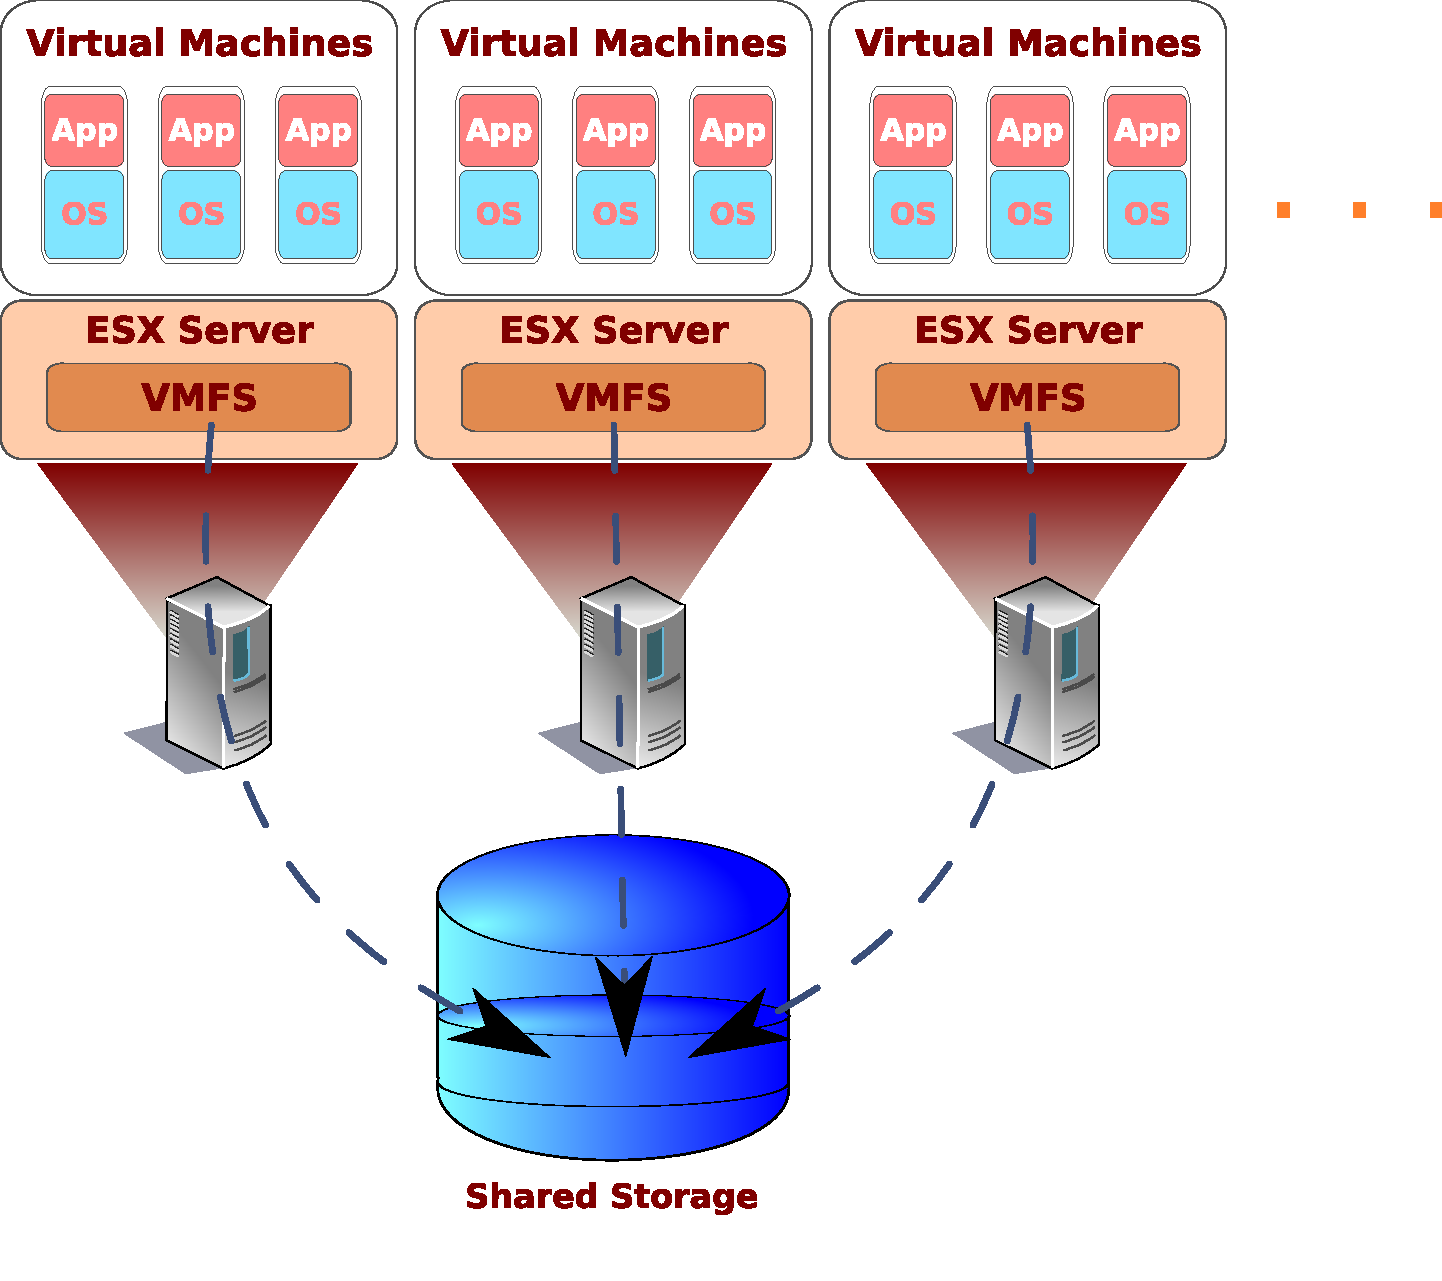
\includegraphics[width=70mm]{figures/vmfs_sysmodel.pdf}
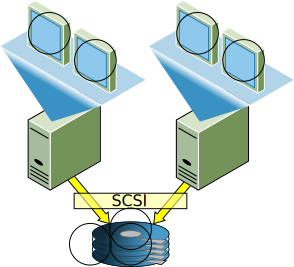
\includegraphics[scale=0.45]{figures/vmfs.pdf}
}
%\vspace{-0.2in}
\caption{Cluster configuration in which multiple hosts
  concurrently access the same storage volume.  Each host runs the
  VMFS file system driver ({\tt \small vmfs3}), the deduplication
  driver ({\tt \small dedup}), and other
  processes such as VMs.}
%\vspace{-0.1in}
\label{fig:vmfs-sysmodel}
\end{figure}


\section{System Overview}
\label{sec:overview}
\label{sec:idea:out-of-band}

\DeDe operates in a cluster setting, as shown in
Figure~\ref{fig:vmfs-sysmodel}, in which multiple hosts are directly
connected to a single, shared SCSI volume and use a file system designed
to permit symmetric and cooperative access to the data stored on the
shared disk.  \DeDe itself runs on each host as a layer on top of the
file system, taking advantage of file system block layout policies and
native support for copy-on-write (COW) blocks.  In this section, we
provide a brief overview of our approach to deduplication and the file
system support it depends on.

% Content hash index

\DeDe uses content hashes to identify potential duplicates,
the same basic premise shared by all deduplication systems.  An index
stored on the shared file system and designed for concurrent access
permits efficient duplicate detection by tracking all known blocks in
the file system by their content hashes.

% Overall scheme

%% As a sketch, file system write operations are intercepted by \DeDe and
%% content hashes are computed while the IO is still in memory. This
%% summary data, called a write log, which constitutes the file system
%% modifications for a particular host is accumulated on each host
%% independently and periodically flushed to the shared disk. Later on,
%% the write log is compared against the deduplication index when, if
%% duplicates are discovered, we can create merge requests to eliminate
%% duplication. These merge requests are in turn, handled by a multitude
%% of hosts independently and asynchronously.

% Out of band

In order to minimize impact on critical file system operations such as
reading and writing to files, \DeDe updates this index \emph{out of
  band}, buffering updates and applying them in large, periodic
batches.  As part of this process, \DeDe detects and eliminates
duplicates introduced since the last index update.  This can be
done as an infrequent, low priority
background task or even scheduled during times of low
activity.  Unlike approaches to deduplication such as
content-addressable storage that integrate content indexes directly
into the file system storage management, \DeDe's index serves solely to
identify duplicate blocks and plays no role in general file system
operations.

\DeDe divides this index update process between hosts.  Each host
monitors its own changes to files in the cluster file system and
stores summaries of recent modifications in on-disk \emph{write logs}.
These logs include content hashes computed in-band, as blocks are
written to disk.  Each host periodically consumes the write logs of files
it has (or can gain) exclusive access to and updates the shared index
\XXX[under exclusive lock] to reflect these recorded modifications. In
the process, it discovers and reclaims any block whose content is
identical to the content of some previously indexed block.  Having
each host participate in the index update process allows the hosts to
divide and distribute the burden of deduplication, while sharing the
index allows hosts to detect duplicates even if they are introduced by
separate hosts. \XXX[Irfan][REVIEW the last line.]

% Resilience

Out-of-band index updates mean \DeDe must be resilient to stale index
entries that do not reflect the latest content of recently updated
blocks.  Indeed, this is essentially unavoidable in a decentralized
setting because of communication delays alone.  While this means \DeDe
generally must verify block contents when updating the index, this
resilience has an important implication: \DeDe's correctness does not
depend on its ability to monitor every write to the file system.  This
has important performance benefits.  First, updates to write logs do
not have to be crash-consistent with updates to file contents, which
both simplifies fault tolerance and allows hosts to buffer updates to
write logs to minimize additional IO.  Second, this allows users to
trade off the CPU and memory overhead of write
monitoring for peak file system performance on a per-file basis.  For
example, a user could simply disable deduplication for VMs that are
performance-critical or unlikely to contain much duplicate data.
Finally, this allows the write monitor to shed work if the system is
overloaded.

% Unique blocks

Because \DeDe operates on a live file system, it specifically
optimizes for \emph{unique} blocks (blocks with no known duplicates).
Unlike \emph{shared} blocks, these blocks remain mutable after
deduplication.  The mutability of unique blocks combined with \DeDe's
resilience to stale index information means these blocks can be
updated in place without the need to allocate space for a copy or to
synchronously update the index.  As a result, deduplication has no
impact on the performance of writing to unique blocks, a highly
desirable property
because these are precisely the blocks that do not benefit from
deduplication.

Similar to some other deduplication work related to virtual
disks~\cite{cas-experiences,nath08hpccas}, \DeDe uses fixed-size
blocks.  Unlike stream-oriented workloads such as backup, where
variable-sized chunks typically achieve better
deduplication~\cite{zhu08datadomain}, our input data is expected to be
block-structured because guest file systems (\eg, ext3, NTFS)
typically divide the disk into fixed-size 4~KB or 8~KB blocks
themselves.  Consistent with this expectation, earlier
work~\cite{nath06vmcas} and our own test results (see
Section~\ref{sec:vmware-vdi-analysis}), we use a block size of 4~KB.

\subsection{Required File System Abstractions}
\label{sec:idea:compare-and-share}

Most approaches to deduplication unify duplicate elimination and
storage management, supplanting the file system entirely.  \DeDe, in
contrast, runs as a layer on top of VMFS, an existing file system.
This layer finds potentially identical blocks and identifies them to
the file system, which is then responsible for merging these blocks
into shared, copy-on-write blocks.

\XXX[Austin][Better transition?]
\DeDe requires the file system to be block oriented and to support
file-level locking.  The file
system block size must also align with the deduplication block size, a
requirement VMFS's default 1~MB block size, unfortunately, does not
satisfy.  Our only non-trivial change to VMFS was to add support for
typical file system block sizes (\ie, 4~KB), as detailed later in
Section~\ref{sec:vmfs}.

Finally, \DeDe requires block-level copy-on-write support, a well
understood, but nevertheless uncommon feature supported by VMFS.
Specifically, it requires an unusual \emph{compare-and-share} operation,
which replaces two blocks with one copy-on-write block after verifying
that the blocks are, in fact, identical (using either bit-wise
comparison or a content hash witness).  Despite the specificity of
this operation, it fits naturally into the structure of block-level
copy-on-write and was easy to add to the VMFS interface.  \DeDe
manipulates file system blocks solely through this interface and has
no knowledge of the underlying file system representation.

There are two noteworthy capabilities that \DeDe does \emph{not}
require of the file system.  First, hosts running \DeDe never modify
the metadata of files they do not have exclusive locks on, as doing so
would require cross-host synchronization and would complicate per-host
metadata caching.  As a result, a host that discovers a duplicate block
between two files cannot simply modify both files to point to the
same block if one of the files is locked by another host.  Instead,
when \DeDe detects a duplicate between files locked by different
hosts, it uses a third file containing a \emph{merge request} as an
intermediary.  One host creates a merge request containing a COW
reference to the deduplicated block, then passes ownership of the
merge request file's lock to the other host, which in turn replaces
the block in its file with a reference to the block carried by the
merge request.

% Section 2.1, 3rd paragraph, last sentence, mentions and italicizes
% merge requests, but doesn't define them (they're described later in
% 2.2).  If you're going to emphasize them, you may as well provide some
% kind of definition or forwarding pointer.

Second, \DeDe does \emph{not} require the file system to expose a
representation of block addresses.  Much like any regular application,
it only refers to blocks indirectly, by their offset in some
locked file, which the file system can resolve into a block
address.  This restricts the design of our index, since it cannot
simply refer to indexed blocks directly.  However, this limitation
simplifies our overall design, since requiring the file system to expose block
addresses outside the file system's own data structures would
interfere with its ability to free and migrate blocks and could result
in dangling pointers.  Worse, any operations introduced to manipulate
blocks directly would conflict with file-level locking and host
metadata caching.

In lieu of referring to blocks by block addresses, \DeDe introduces a
\emph{virtual arena} file.  This is a regular file in the file system,
but it consists solely of COW references to shared blocks that are
present in at least one other file.  This file acts as an alternate
view of all shared blocks in the system: \DeDe identifies shared
blocks simply by their offsets in the virtual arena file, which the
file system can internally resolve to block addresses using regular
address resolution.

Because \DeDe builds on the underlying file system, it inherits the
file system's block placement policy and heuristics.  If the
underlying file system
keeps file blocks sequential, blocks will generally remain sequential
after deduplication.  Shared blocks are likely to be sequential with
respect to other blocks in at least one file, and common sequences of
shared blocks are likely to remain sequential with respect to each
other.  Furthermore, the placement and thus sequentiality of unique
blocks is completely unaffected by the deduplication process; as a
result,
%
% not only is IO performance to individual unique blocks
% unaffected after deduplication because they do not require copying,
% but sequential IO performance across spans of unique blocks is also
% maintained.
%
deduplication does not affect IO performance to individual unique
blocks because they do not require copying, and it maintains
sequential IO performance across spans of unique blocks.

\subsection{VMFS}
\label{sec:vmfs}

Many of the design decisions in \DeDe were influenced by the design of
its substrate file system, VMFS.  VMFS is a coordinator-less cluster
file system~\cite{vmfsdatasheet} designed to allow hosts to
cooperatively maintain a file system stored on a shared disk. In this
section, we provide a quick overview of how VMFS addresses and
manages concurrent access to its resources in order to provide better
context for the design of \DeDe.

VMFS organizes the shared disk into four different resource pools:
inodes, pointer blocks, file blocks, and sub-blocks.  Inodes and
pointer blocks play much the same role as in traditional UNIX file
systems, storing per-file metadata and pointers to the blocks
containing actual file content.  File blocks and sub-blocks both store
file content, but are different sizes, as discussed below.  The
divisions between these pools are currently fixed at format time and
can only be expanded by adding more storage, though this is not a
fundamental limitation.  In each pool,
resources are grouped into \emph{clusters}. The header for each cluster
maintains metadata about all of its contained resources; most
importantly, this includes a reference count for each
individual resource and tracks which resources are free and which are
allocated.

In order to support concurrent access by multiple hosts to file and
resource data, VMFS uses a distributed lock manager.
Unlike most cluster file systems, which use an
IP network for synchronization, VMFS synchronizes all file system
accesses entirely through the shared disk itself using on-disk locks.
VMFS ensures atomic access to on-disk lock structures themselves using
SCSI-2-based LUN reservations to guard read-modify-write critical
sections.  In addition to taking advantage of the reliability of
storage area networks, using the same means to access both file system
state
and synchronization state prevents ``split brain'' problems typical of
IP-based lock managers in which multiple hosts can access the file
system state but cannot communicate locking decisions with each other.

VMFS protects file data from concurrent access by associating a
coarse-grain lock with each file that covers all of a file's metadata
(its inode and pointer blocks) as well as all of the file blocks and
sub-blocks comprising the file's content.  Files in VMFS tend to be
locked for long durations (\eg, a VM's disk files are locked as long
as the VM is powered on). \DeDe respects file system locking by
partitioning the deduplication process according to which hosts hold
which file locks.
% ... so \DeDe must deduplicate data blocks in locked files in a
% manner that is both efficient and respects the file system locking
% protocol.

VMFS protects resource metadata using per-cluster locks.  Thus,
allocation and deallocation of resources must lock all clusters
containing any of the resources involved.  The number of resources
packed per cluster reflects a trade-off between locking overhead and
cross-host cluster lock contention.  Higher cluster density allows
hosts to manipulate more resources with fewer locks, but at the cost of
increased lock contention.  Since \DeDe stresses the sub-block resource pool
more than typical VMFS usage, we increase the sub-block cluster
density from 16 to 128 resources per cluster, but otherwise use the
default VMFS densities.

% JL: agree, removed
% \XXX[Austin][This is probably good to talk about, but doesn't fit in
% very nicely.]
% Resource allocation in VMFS is similar to that of a next-fit memory
% allocator~\cite{next-fit}.  Each host uses a hash of its own MAC
% address to pick an initial cluster from which to allocate resources
% when mounting the file system.  The host allocates from this cluster
% until exhausting it and moving on to the next cluster.  The staggering
% of initial allocation clusters combined with lingering until clusters
% are exhausted helps to minimize cross-host lock contention, but can
% negatively impact sequentiality.

\begin{figure}[t]
\centerline {
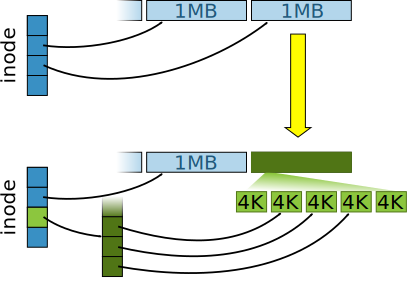
\includegraphics[scale=0.45]{figures/mixed.pdf}
}
\caption{Mixed block sizes allow any 1~MB file block to be divided into
  256 separate 4~KB sub-blocks.}
\label{fig:mixed-block-sizes}
\end{figure}

VMFS maintains two separate resource types for storing file content:
file blocks and sub-blocks.  File sizes in VMFS typically fit a
bimodal distribution.  Virtual machine disks and swap files are
usually several gigabytes, while configuration and log files tend to
be a few kilobytes.  Because of this, VMFS uses 1~MB file blocks to
reduce metadata overhead and external fragmentation for large files,
while for small files, VMFS uses smaller
sub-blocks to minimize internal fragmentation.
\DeDe must be able to address individual 4~KB blocks in order to COW
share them, so we configure VMFS with 4~KB sub-blocks.
Furthermore, rather than simply eschewing the efficiency of 1~MB blocks
and storing all file content in 4~KB blocks, we extend VMFS to
support \emph{mixed block sizes}, depicted in
Figure~\ref{fig:mixed-block-sizes}, so that \DeDe can address
individual
4~KB blocks of a file when it needs to share a duplicate block, but
when possible still store unique regions of files in efficient 1~MB
blocks.  This change introduces an optional additional pointer block
level and allows any file block-sized region to be broken into 256 
separate 4~KB blocks, which, in turn, add up to the original file
block.  This can be done
dynamically to any 1~MB block based on deduplication decisions,
and leaves address resolution for other data intact and efficient.

Beyond these unusual block sizes, VMFS supports a number of other
uncommon features.  Most important to \DeDe is support for block-level
copy-on-write (COW).  Each file or sub-block resource can be
referenced from multiple pointer blocks, allowing the same data to be
shared between multiple places in multiple files.  Each reference to a
shared resource is marked with a COW bit, indicating that any attempts
to write to the resource must make a private copy in a freshly
allocated resource and write to that copy instead.  Notably, this COW
bit is associated with each \emph{pointer} to the resource, not with the
resource itself.  Otherwise, every write operation would need to take
a cluster lock to check the COW bit of the destination block, even if
the block was not COW.  However, as a result, sharing a block between
two files requires file locks on \emph{both} files, even though only
one of the references will change.  Thus, \DeDe must use merge
requests for all cross-host merging operations.

VMFS forms the underlying substrate of \DeDe and handles critical
correctness requirements such as specializing COW blocks and
verifying potential duplicates, allowing \DeDe to focus on
duplicate detection.  Virtual arenas and merge requests
allow \DeDe to achieve complex, decentralized manipulations of the
file system structure without knowledge of the file system
representation, instead using only a few general-purpose interfaces.

% VMFS has attained significant market acceptance with a majority of
% VMware ESX Server users deploying it in their environments to run
% enterprise production workloads. As such, VMFS provided a well-tested
% base to develop our \DeDe prototype on top of.

% Each system file has a resource file header, followed by multiple
% recurring sequences of densely packed resource clusters (along with
% their associated disk locks) and the resources they are comprised of.
% The resource file header describes the number of resources per
% cluster, number of clusters per cluster group, size of each resource,
% total number of resources and cluster groups and other information
% needed to manage the specific resource type.  The resource clusters
% have a resource bitmap to track resource allocation and deallocation
% and a two byte reference counter per resource to track the total
% number of references to a specific resource (which is used to
% implement snapshots). Resources are deallocated and marked free in the
% bitmap only when their corresponding reference counters drop to zero.

% The inode structure in VMFS is akin to that of a traditional UNIX file
% system inode with pointers to fixed-size blocks. Due to the fairly
% large file block sizes, the design does not support more than a
% single-level of indirection via pointer-blocks
% (Section~\ref{sec:mixed-block-sizes} describes why this limitation had
% to be overcome for \DeDe).  As a performance optimization, VMFS embeds
% the copy-on-write flag in the file metadata itself instead of the
% block metadata. This implies that even if modifying file A to point to
% a block in file B, a lock might still be needed on file B to make its
% pointer COW.  Another important design aspect that has performance
% implications for copy-on-write with VMFS (and \DeDe) is the fact that
% resource clusters (block metadata) do not hold a back reference to the
% holder(s) of the resource (file metadata). This implies that if there
% are two copy-on-write references to the same block from file A and
% file B, deletion of file B will not automatically cause the
% copy-on-write flag in file A's metadata to be unset. A subsequent
% write will still incur the penalty of a copy-on-write.

% \subsection{Content Hashing}
% \label{sec:content-hashing}

% \DeDe uses \shaone~\cite{fips-180-2} to fingerprint contents of
% blocks. To date, there aren't any known hash collisions from using the
% \shaone function and it is generally considered a collision-resistant
% crypto secure hash. However, there is debate about whether history
% will repeat itself with this function eventually getting broken in a
% computationally feasible implementation~\cite{henson-compare-by-hash,
%   black-compare-by-hash}. Whereas we hold that using \shaone or similar
% function is safe for our purposes, we chose to keep the flexibility in
% \DeDe to perform bit-by-bit comparisons before deduplicating. It is
% worth noting that the \shaone hashes are used in our system to simply
% identify duplicates and not to address them during normal
% runtime. \DeDe only supports traditional file system location
% addressing using the $\tup<\text{filename},\text{offset}>$ tuple. As
% such, if \shaone must be replaced, our system can be safely
% upgraded by installing a new hash function and reconstructing the
% index, a process during which the file system can continue to execute
% without interruption.

%% a worst-case workload for \DeDe is encrypted guest fileystems,
%% nevertheless \DeDe can provide good deduplication peformance for a
%% variety of workloads.




% -*- TeX-master: "paper.tex"; TeX-PDF-mode: t; ispell-local-pdict: "words" -*-



\section{Design and Implementation}
\label{sec:design}

In this section, we provide details of the design and implementation
of \DeDe's best-effort write
monitoring subsystem and the out-of-band indexing and duplicate
elimination process.

\subsection{Write Monitoring}
\label{sec:idea:stale-wlog}

%%%%%%%%%%%%%%%%%%%%%%%
%%%% Figure %%%%%%%%%%%
%%%%%%%%%%%%%%%%%%%%%%%

\begin{figure}[t]
\centerline {
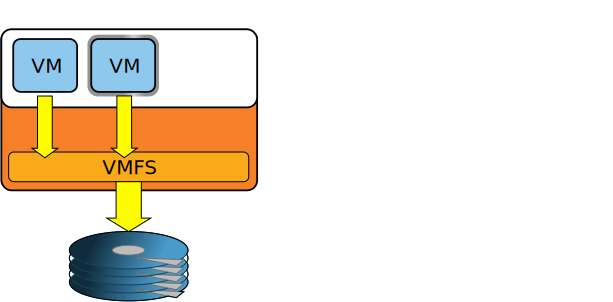
\includegraphics[scale=0.45]{figures/writemon.pdf}
}
%\vspace{-0.2in}
\caption{Only a lightweight kernel module lies
  in the IO critical path, opportunistically calculating hashes of
  blocks while they are still in memory. A userspace daemon ({\tt
    \small dedupd}) flushes write logs to disk periodically. Duplicate
  detection and elimination occur out of band.}
%\vspace{-0.1in}
\label{fig:write-monitoring}
\end{figure}

%%%%%%%%%%%%%%%%%%%%%%%
%%%% /Figure %%%%%%%%%%
%%%%%%%%%%%%%%%%%%%%%%%

Each host runs a \emph{write monitor}, as shown in
Figure~\ref{fig:write-monitoring}, which consists of a lightweight
kernel module ({\tt \small dedup}) that monitors all writes by that host
to files in the file system and a userspace daemon ({\tt \small dedupd}) that
records this information to logs stored in the shared file system.
The write monitor is the only part of the system that lies in the
IO critical path of the file system, so the write monitor itself must
incur as little additional disk IO and CPU overhead as possible.

% We divide deduplication into separate monitoring and merging processes
% in order to minimize the impact of the system on regular file system
% reads and writes, so we must ensure that the write monitor itself
% incurs as little additional disk IO and CPU overhead as possible.

The kernel module provides the userspace daemon with a modification
stream indicating, for each write done by the host: the file modified,
the offset of the write, and the \shaone hashes of all modified
blocks.  While the in-band CPU overhead of the monitor could have been
virtually eliminated by computing these hashes lazily (\eg, at
indexing time), this would have required reading the modified blocks
back from disk, resulting in a large amount of additional random IO.
We opted instead to eliminate the extra IO by computing these hashes
while the blocks were in memory, though the trade-off between run-time
CPU overhead and deduplication-time IO overhead could be set
dynamically by user-defined policy.

The userspace daemon divides the modification stream by file,
aggregates repeated writes to the same block, and buffers this
information in memory, periodically flushing it to individual write
log files associated with each regular file.  These write logs are
stored on the shared file system itself, so even if
a host fails or transfers ownership of a file's lock, any other host
in the system is capable of reading logs produced by that host and
merging information about modified blocks into the index.

The daemon can safely buffer the modification stream in memory because
the index update process is designed to deal with stale
information.  Without this, write logs would have to be consistent
with on-disk file state, and each logical write to the file system
would result in at least
two writes to the disk.  Instead, buffering allows our system to
absorb writes to over 150~MB of file blocks into a single infrequent
1~MB sequential write to a log file.  This is the only additional IO
introduced by the write monitor.
% (/ (/ (* (/ (* 1024 1024) (+ 20 4)) 4096) 1024) 1024)
% XXX One word overflow, but prevents orphan

Similarly, we rely on the best-effort property of write monitoring to
minimize IO in the case of partial block writes.  If a write
to the file system does not cover an entire block, the monitor simply
ignores that write, rather than reading the remainder of the block
from disk simply to compute its hash.  In practice, this is rarely a
problem when writes originate from a virtual machine, because guest
operating systems typically write whole guest file system blocks,
which are generally at least 4~KB.\footnote{Unfortunately, owing to an
  ancient design flaw in IBM PC partition tables, guest writes are not
  necessarily \emph{aligned} with \DeDe blocks.
  Section~\ref{sec:vmware-vdi-analysis} has a more detailed
  analysis of this.}
% USENIX technically forbids footnotes, but this doesn't make sense as
% an endnote and I've seen USENIX papers use footnotes before.

Write monitoring can be enabled or disabled per file.
If the performance of some VM is too critical to incur the
overhead of write monitoring or if the system administrator has
a priori knowledge that a VM's duplication ratio is small, such VMs
can be opted out of deduplication.

\subsection{The Index}

%%%%%%%%%%%%%%%%%%%%%%%
%%%% Figure %%%%%%%%%%%
%%%%%%%%%%%%%%%%%%%%%%%

% \begin{figure*}
% \centerline {
% 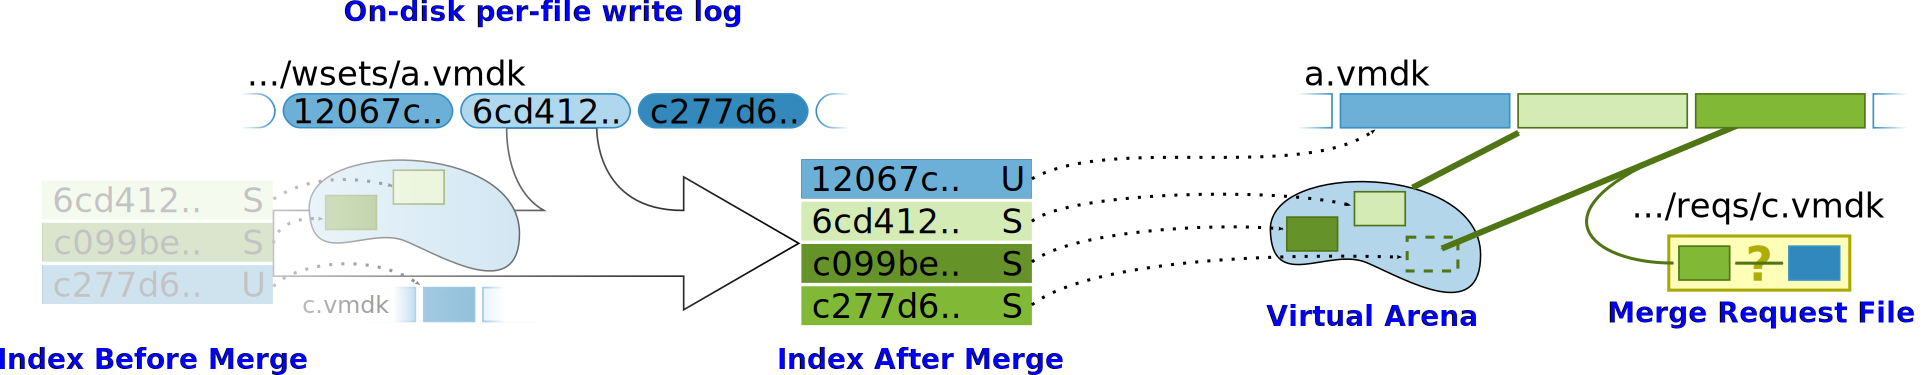
\includegraphics[width=6.0in]{figures/indexing-merging.pdf}
% }
% %\vspace{-0.2in}
% \caption{Indexing and Merging: The index is a map from hash to
%   offsets. For shared blocks (S), the offset is in the virtual arena
%   file whereas for unique blocks (U), it is in a reguar file. Hosts
%   process write logs for their files against the index and zip the two
%   together. The left side of the figure is before a merge operation
%   and the right is after. The entry in the index for c277d6... was
%   converted from a hint unique entry (U) to a shared one (S). As part
%   of that, the host performing that operation left a merge request
%   for whichever host owned file c.vmdk.}
% %\vspace{-0.1in}
% \label{fig:indexing-merging}
% \end{figure*}

%%%%%%%%%%%%%%%%%%%%%%%
%%%% /Figure %%%%%%%%%%
%%%%%%%%%%%%%%%%%%%%%%%

% \begin{comment}
%   The index maintains both shared and unique block locators.

%   Index updates occur in large, periodic batches, once enough writes
%   to the file system have accumulated.  Because of this, the structure
%   is optimized for concurrent, batch update.

%   All blocks referenced by the arena, modulo uncollected garbage
%   blocks, are also referenced by at least one regular file in the file
%   system, so the arena can be thought of as consisting solely of
%   metadata.  The arena gives our system a stable way to refer to
%   blocks without the need for the file system to expose raw block
%   pointers and all of their dangers.  Whenever we add a block to the
%   arena, it remains where it originally was on disk (ideally,
%   sequential with the original containing file), allowing us to take
%   advantage of the file system's placement policy.
% \end{comment}

The shared on-disk index tracks all known blocks in the file system by
their content hashes.  As discussed in
Section~\ref{sec:idea:out-of-band}, each host updates this index
independently, incorporating information about recent block
modifications from the write logs in large batches on a schedule set
by user-defined policy (\eg, only during off-peak hours). A match
between a content hash in the index and that of a recently modified
block indicates a potential duplicate that must be verified and
replaced with a copy-on-write reference to the shared block.

% \XXX[Austin][Batch updates amortize the cost of synchronization on the
% index files]

The index acts as an efficient map from hashes to block locations.
Because \DeDe treats unique blocks (those with only a single
reference) differently from shared blocks (those with multiple
references), each index entry can likewise be in one of two states,
denoted $\text{Unique}(H,f,o)$ and $\text{Shared}(H,a)$.  An index
entry identifies a unique block with hash $H$ by the inumber $f$ of
its containing file and its offset $o$ within that file.  Because
index updates are out-of-band and unique blocks are mutable, these
entries are only \emph{hints} about a block's hash.  Thus, because a mutable
block's contents may have changed since it was last indexed, its
contents must be verified prior to deduplicating it with another
block.  Shared blocks, on the other hand, are marked COW and thus
their content is guaranteed to be stable.  The index identifies each
shared block by its offset $a$ in the index's \emph{virtual arena},
discussed in the next section.

\subsubsection{Virtual Arena}

When duplicate content is found, \DeDe reclaims all but one of the duplicates
and shares that block copy-on-write between files.  Because hosts can
make per-file, mutable copies of shared blocks at any time without
updating the index, we cannot simply identify shared blocks by their
locations in deduplicated files, like we could for unique blocks.  The
index needs a way to refer to these shared blocks that is stable
despite shifting references from deduplicated files.  As
discussed earlier, \DeDe cannot simply store raw block addresses in the
index because exposing these from the file system presents numerous
problems.  Instead, we introduce a virtual arena file as an
additional layer of indirection that provides stable identifiers for
shared blocks without violating file system abstractions.

\iffalse
% Not really happy with this figure yet
\begin{figure}
  \centering
  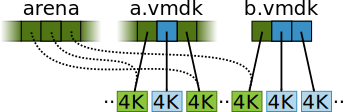
\includegraphics[scale=0.45]{figures/virtualarena.pdf}
  \caption{The virtual arena file appears to contain all shared blocks
    in the file system, but only by way of reference to blocks shared
    by other files.}
  \label{fig:virtual-arena}
\end{figure}
\fi

The virtual arena is a regular file, but unlike typical files, it
doesn't have any data blocks allocated specifically for it (hence, it
is virtual).  Rather, it serves as an alternate view of all shared
blocks in the file
system.  In this way, it is very different from the arenas used in
other deduplication systems such as Venti~\cite{quinlan02venti}, which
store actual data blocks addressed by content addresses.

In order to make a block shared, a host introduces an additional COW
reference to that block from the virtual arena file, using the same
interface that allows blocks to be shared between any two
files.  Apart from uncollected garbage blocks, the virtual arena
consumes only the space of its inode and any necessary pointer
blocks.  Furthermore, this approach takes advantage of the file
system's block placement policies: adding a block to the virtual arena
does \emph{not} move
it on disk, so it is likely to remain sequential with the original
file.

The index can then refer to any shared block by its \emph{offset} in
the virtual arena file, which the file system can internally resolve
to a block address, just as it would for any other file.  The virtual
arena file's inode and pointer block structure exactly form the
necessary map from the abstract, stable block identifiers required by
the index to the block addresses required by the file system.

\subsubsection{On-disk Index Representation}
\label{sec:index:representation}

\DeDe stores the index on disk as a packed list of entries,
sorted by hash.  Because \DeDe always updates the index in large
batches and since the hashes of updates exhibit no spatial
locality, our update process simply scans the entire index file
linearly in tandem with a sorted list of updates, merging the two lists
to produce a new index file.  Despite the simplicity of this
approach, it outperforms common index structures optimized for
individual random accesses (\eg, hash tables and B-trees) even if the
update batch size is small.  Given an average index
entry size of $b$ bytes, a sequential IO rate of $s$ bytes per second,
and an average seek time of $k$ seconds, the time required to apply
$U$ updates using random access is $Uk$, whereas the time to
scan and rewrite
an index of $I$ entries sequentially is $\nicefrac{2Ib}{s}$.  If the
ratio of the batch size to the index size exceeds
$\nicefrac{U}{I} = \nicefrac{2b}{sk}$, sequentially rewriting the
entire index is faster than applying each update individually.
For example, given an entry size of $23$
bytes and assuming a respectable SAN array capable of 150~MB/s and
8~ms seeks, the batch size only needs to exceed $0.004\%$ of the index
size.  Furthermore, hosts defer index updates until the batch size
exceeds some fixed fraction of the index size (at least $0.004\%$), so
the amortized update cost remains
constant regardless of index size.

% b = record size in bytes
% s = sequential IO rate in bytes per second
% k = average seek time in seconds
% |I| = index size in bytes
% n = number of update in a batch

% Where is the inflection point?
% * seconds for sequential update = 2*|I|/s
% * seconds for random update = nk
% * at the inflection point, 2*|I|/s = nk
% * rearrange to get
%   nb/|I| = the ratio of update size to index size
%          = 2b/sk

% RAID'd SAN
% (let* ((K 1024) (b 23) (s (* 150 K K)) (k 8e-3)) (* 100 (/ (* 2 b) (* s k))))

% Average, good disk
% (let* ((K 1024) (b 23) (s (* 70 K K)) (k 8e-3)) (* 100 (/ (* 2 b) (* s k))))

% Worst case
% (let* ((K 1024) (b 23) (s (* 50 K K)) (k 5e-3)) (* 100 (/ (* 2 b) (* s k))))

In order to allow access to the index to scale with the number of
hosts sharing the file system, while still relying on file locking to
prevent conflicting index access, hosts {\it shard} the index into multiple
files, each representing some subdivision of the hash space.  Once the
time a host takes to update a shard exceeds some threshold, the next
host to update that shard will split the hash range covered by the
shard in
half and write out the two resulting sub-shards in separate files.  This
technique mirrors that of extensible
hashing~\cite{fagin79extendiblehashing}, but instead of bounding the
size of hash buckets, we bound the time required to update them.
Combined with file locking, this dynamically adjusts the concurrency
of the index to match demand.

\subsection{Indexing and Duplicate Elimination}

As the index update process incorporates information about recently
modified blocks recorded in the write logs, in addition to detecting
hash matches that indicate potential duplicates, it also performs
the actual COW sharing operations to eliminate these duplicates.  The
duplicate elimination process must be interleaved with the index
scanning process because the results of block content verification can
affect the resulting index entries.
% We begin with an explanation of this process
% assuming only a single host, then describe the changes necessary to
% support multiple hosts, and finally discuss garbage collection.

In order to update the index, a host sorts the recent write
records by hash and traverses this sorted list of write records in
tandem with the sorted entries in the index.  A matching hash between
the two indicates a potential duplicate, which is handled differently
depending on the state of the matching index entry.
Figure~\ref{fig:index-states} gives an overview of all possible
transitions a matching index entry can undergo, given it current
state.

\captionsetup[subfloat]{subrefformat=parens}

\begin{figure}
  \centering
  %
  \subfloat[When the hash $H$ of the block at offset $o$ in file $f$
  is not in the index, a new unique entry is added.]
           {\label{fig:new-unique}
             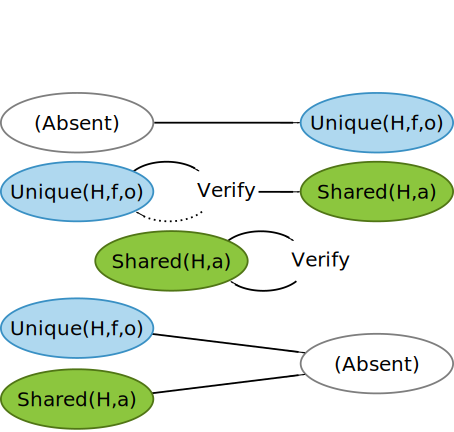
\includegraphics[scale=0.45,viewport=0 220 364
               275,clip]{figures/indexstates.pdf}} \\
%
  \subfloat[When a second occurrence of hash $H$ is found and the
    block's content passes verification, we place it in the virtual
    arena and upgrade the index entry to shared.]
           {\label{fig:unique-to-shared}
             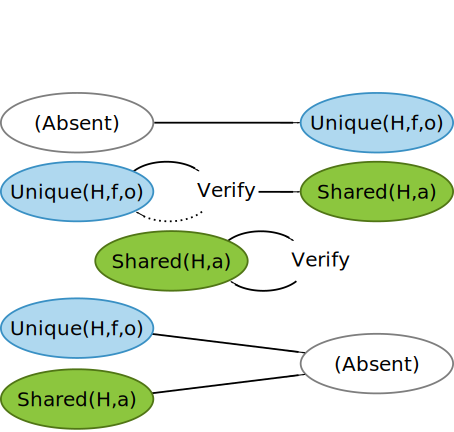
\includegraphics[scale=0.45,viewport=0 165 364
               220,clip]{figures/indexstates.pdf}} \\
%
  \subfloat[When a duplicate of a shared block is found, we
    verify its contents and replace the block with a reference to the
    existing shared block.]
           {\label{fig:shared-to-shared}
             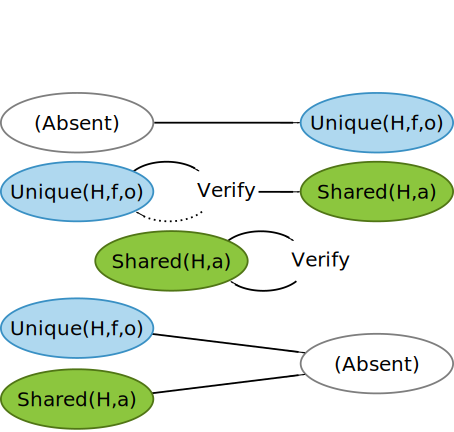
\includegraphics[scale=0.45,viewport=0 110 364
               165,clip]{figures/indexstates.pdf}} \\
%
  \subfloat[Unique entries are garbage collected when the indexing
    process finds a write record to that block with a different hash.
    Shared entries are garbage collected when only the reference from
    the virtual arena remains.]
           {\label{fig:gc}
             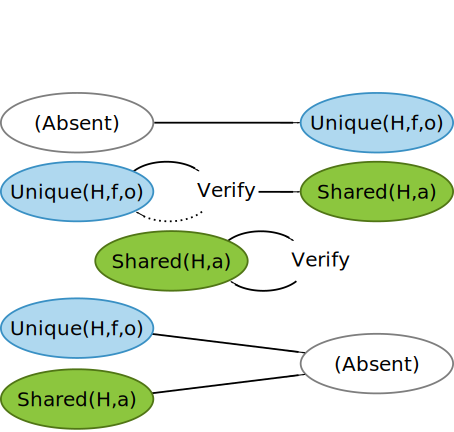
\includegraphics[scale=0.45,viewport=0
               0 364 110,clip]{figures/indexstates.pdf}} \\
%
  \caption{All possible updates to an index entry.}
  \label{fig:index-states}
\end{figure}

When \DeDe detects a potential duplicate, it depends on the file
system's compare-and-share operation, described in
Section~\ref{sec:idea:compare-and-share}, to atomically verify that
the block's content has not changed and replace it with a COW
reference to another block.  Based on user-specified policy, this
verification can either be done by reading the contents of the
potential duplicate block and ensuring that it matches the expected
hash (\ie, compare-by-hash), or by reading the contents of \emph{both}
blocks and performing a bit-wise comparison (\ie, compare-by-value).
If the latter policy is in effect, hash collisions reduce \DeDe's
effectiveness, but do \emph{not} affect its correctness.  Furthermore,
because hashes are used solely for finding potential duplicates, if
\shaone is ever broken, \DeDe has the unique capability of gracefully
switching to a different hash function by simply rebuilding its index.
The content verification step can be skipped altogether if a host can
prove that a block has not changed; for example, if it has held the
lock on the file containing the block for the entire duration since
the write record was generated and no write records have been dropped.
While this is a fairly specific condition, it is often met in \DeDe's
target setting because locks on VM disks are usually held for very
long durations.

\subsubsection{Single Host Indexing}

We begin with an explanation of the index update process assuming only
a single host with exclusive access to the file system.  In a single
host design, the host can modify the metadata of any file.  We lift
this assumption in the next section, where we extend the process to
support multiple hosts.

Any write record without a corresponding hash in the index indicates a
new, unique block.  Even though this write record may be stale,
because index entries for unique blocks are only hints, it is
safe to simply add the new unique block to the index without verifying
the block's content, performing an \emph{absent-to-unique}
transition as shown in
Figure~\subref*{fig:new-unique}.  This single
sequential, buffered write to the index is the only IO incurred when
processing a new unique block.

When a write record's hash corresponds to an index entry for a
unique block, then the host attempts to share both blocks (freeing one
of them in the process) and upgrade the index entry to refer to the
shared block.  This \emph{unique-to-shared} transition is shown in
Figure~\subref*{fig:unique-to-shared}.  However,
because the write record and index entry may both be stale,
the host must verify the contents of both blocks before actually
sharing them.  Assuming this verification succeeds, the file system
replaces both blocks with a shared block and the host inserts
this block into the virtual arena and upgrades the index entry to
refer to the new, shared block.

Finally, if a write record's hash matches an index entry for a
shared block, then the host attempts to eliminate this newly detected
potential duplicate, performing a \emph{shared-to-shared} transition
as shown in
Figure~\subref*{fig:shared-to-shared}.  Because
the write record may be stale, it first verifies that the content of
the potential duplicate has not changed.  If this succeeds, then this
block is freed and the reference to the block is replaced with a
reference to the shared block found via the virtual arena.

\subsubsection{Multi-Host Indexing}

Extending the index update process to multiple hosts, we can no longer
assume that a host will have unfettered access to every file.  In
particular, hosts can only verify blocks and modify block pointers in
files they hold exclusive locks on.  As a result, indexing \emph{must}
be distributed across hosts.  At the same time, we must minimize
communication between hosts, given the cost of communicating via the
shared disk.  Thus, sharing of blocks is done without
any blocking communication between hosts, even if the blocks involved
are in use by different hosts.

In the multi-host setting, the write logs are divided amongst the
hosts according to which files each host has (or can gain) exclusive
access to.  While this is necessary because hosts can only process
write records from files they hold exclusive locks on, it also serves
to divide the deduplication workload between the hosts.

Absent-to-unique transitions and shared-to-shared transitions are
the same in the multi-host setting as in the single host setting.
Adding a new, unique block to the
index requires neither block verification, nor modifying block
pointers.  Shared-to-shared transitions only verify and rewrite blocks
in the file referenced by the current write log, which the host
processing the write log must have an exclusive lock on.

Unique-to-shared transitions, however, are complicated by the
possibility that the file containing the
unique block referenced by the index may be locked by some host other
than the host processing the write record.  While this host
may not have access to the indexed block, it does
have access to the block referred to by the write log.  The host
verifies this
block's content and promotes it to a shared block by adding it to the
virtual arena and upgrading the index entry accordingly.  However, in
order to reclaim the originally indexed block, the host must
communicate this deduplication opportunity to the host holding the
exclusive lock on the file containing the originally indexed block
using the associated merge request file.  The host updating
the index posts a merge request for the file containing the originally
indexed block.  This request contains not only
the offset of the unique block, but also another COW reference to the
shared block.  Hosts periodically check for merge requests to the files
they have exclusive locks on, verifying any requests they
find and merging blocks that pass verification.  The COW
reference to the shared block in the merge request allows hosts to
process requests without accessing the arena.

% Hosts periodically check the merge logs of
% the files they have exclusive locks on, verifying any merge hints that
% they find and merging blocks that pass verification.  Including a COW
% reference to the shared block in the merge hint allows hosts to
% process merge logs without locking the arena.

\subsubsection{Garbage Collection}

As the host scans the index for hash matches, it also
garbage collects unused shared blocks and stale index entries, as
shown in Figure~\subref*{fig:gc}.  For each 
shared block in the index, it checks the file system's reference count
for that block.  If the block is no longer in use, it will have only a
single reference (from the virtual arena), indicating that it can be removed
from the virtual arena and freed.  In effect, this implements a simple form of
weak references without modifying file system semantics.  Furthermore,
this approach allows the virtual arena to double as a victim cache before
garbage collection has a chance to remove unused blocks.

Unique blocks do not need to be freed, but they can leave behind stale
index entries.  Hosts garbage collect these by removing any index entries
that refer to any block in any of the write records being processed by
the host.  In the presence of dropped write records, this may not remove
all stale index entries, but it will ensure that there is at most one
index entry per unique block.  In this case, any later write or potential
duplicate discovery involving a block with a stale index entry will
remove or replace the stale entry.  The garbage collection process
also check for file truncations and deletions and removes any
appropriate index entries.




% \subsection{Index Merging}

% Merging is the process by which an index is updated to include newly
% written data from write logs. In \DeDe, the merging task must be
% distributed across hosts. We avoid involving multiple hosts
% simultaneously because communications is expensive and introduces
% complex failure modes.  So, sharing of blocks is done without
% interactive involvement of multiple hosts, even if the blocks involved
% are in use by different hosts.

% The pending updates to the index stored in the write logs are divided
% amongst the hosts according to which files each host has exclusive
% access to.  While this is necessary because hosts can only process
% updates from files they hold exclusive locks on, it also serves to
% divide the deduplication workload between the hosts.  Once a host has
% accumulated enough pending updates, it updates the index, eliminates
% duplicate blocks, and garbage collects the shared block arena in one
% interleaved process.\XXX[mention figure]

% Figure~\ref{fig:indexing-merging} shows the main parts of the system
% before (left) and after a merge operation. Hosts process write logs
% for their files against the index and zip the two together. Let's take
% an example of the entry in the index corresponding to the hash
% c277d6... This entry was added as a unique block from c.vmdk by host A
% at some point in time in the past. As part of the depicted merge, the
% write log for a.vmdk from host B also had the same block. So, host B
% converted it from a unique entry (U) to a shared one (S) and added it
% to some unoccupied offset in the arena and stored that offset in
% index entry. As part of that operation, c.vmdk couldn't be updated because
% it was still locked by host B. Therefore host A left a merge request
% for host B in a merge request file. Later on, host B picked up the
% merge request and after verification backed reclaimed its duplicate
% block by changing its file pointer to the same as in the virtual
% arena.

% \XXX[ For shared blocks (S), the
% offset is in the virtual arena file whereas for unique blocks (U), it
% is in a reguar file.]

% The linear index representation affords a simple update process: the
% host sorts the updates by hash and traverses the sorted updates in
% tandem with the sorted on-disk index, zipping the two structures
% together to produce the updated index.
% % For a given updated block, there are three possibilities: the
% % block's hash may simply be missing from the index, it may refer to a
% % shared block, or it may refer to a unique block.
% Each update results in either a local merging operation or a
% cross-host merging operation, depending on the presence and type of
% the corresponding index record.

% \XXX[I still feel like this is too hard to wrap one's head around.  We
% need a better overview of index merging to orient the reader before
% giving the details.]

% \subsubsection{Local Merging}

% When an updated block is either a new unique block or another
% duplicate of an already shared block, then the index update can be
% done entirely local to the host performing deduplication.

% If an updated block's hash is missing from the index, then that block
% is a new, unique block.  Even though the update record might be stale,
% unique index records can also be stale, so a host can simply add a new
% unique record for the block to the index without verifying the block's
% hash.  This single sequential, buffered write to the index is the only
% IO incurred by a unique block update.

% If the updated block's hash corresponds to a shared block in the
% index, then an existing, copy-on-write version of the block is already
% available in the arena.  The host verifies that the block's contents
% haven't changed since the update record (comparing either by hash or
% by value) and merges the block from the arena into the original file
% by overwriting the block pointer in the original file with a copy of
% the block pointer from the arena, freeing the block from the original
% file in the process.

% \subsubsection{Cross-Host Merging}

% The transition from unique to shared is complicated by the possibility
% that the file containing the previously unique block and the file
% containing the newly found duplicate may be locked by different hosts.
% Communications between hosts is expensive because we limit ourselves
% to communicating only through shared files on disk, and any
% synchronous communication would introduce complex failure modes.
% Instead, we avoid entirely the simultaneous involvement of multiple
% hosts through asynchronous \emph{merge hints}.  Much like write log
% files, each regular file may have a corresponding merge log containing
% hints of potential deduplication opportunities suggested by other
% hosts.

% When an updated block's hash corresponds to a unique block in the
% index, the block's contents are no longer unique and the block must be
% shared.  While the host creating the shared block may not have access
% to the unique block referenced by the index, it does have access to
% the newly discovered duplicate block.  It makes this block shared by
% verifying its hash, making a COW reference to the block from a freshly
% allocated slot in the arena, and updating the index to replace the
% unique record with a shared record.  It then initiates a cross-host
% merge by posting a merge hint containing the address of the unique
% block that was referenced by the index as well as a COW reference to
% the newly shared block.  Hosts periodically check the merge logs of
% the files they have exclusive locks on, verifying any merge hints that
% they find and merging blocks that pass verification.  Including a COW
% reference to the shared block in the merge hint allows hosts to
% process merge logs without locking the arena. Our hinting scheme is
% similar to memory deduplication hints in~\cite{waldspurger-osdi}.


% \subsection{Mixed VMFS Block Sizes}
% \label{sec:mixed-block-sizes}
% %%%%%%%%%%%%%%%%%%%%%%%
% %%%% Figure %%%%%%%%%%%
% %%%%%%%%%%%%%%%%%%%%%%%
% 
% \begin{figure}[t]
% (a)
% \centerline {
% 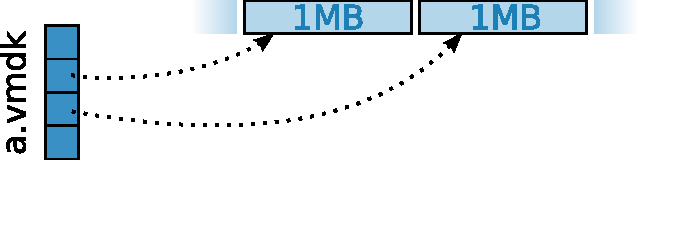
\includegraphics[width=60mm]{figures/1MBsize.pdf}
% }
% (b)
% \centerline {
% 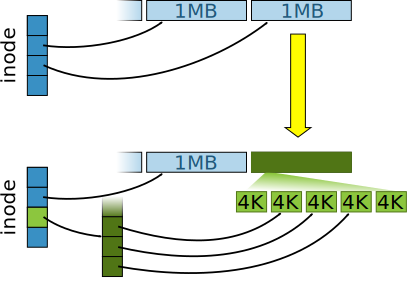
\includegraphics[width=60mm]{figures/mixed.pdf}
% }
% %\vspace{-0.2in}
% \caption{Mixed Block Sizes}
% %\vspace{-0.1in}
% \label{fig:mixed-block-sizes}
% \end{figure}
% 
% %%%%%%%%%%%%%%%%%%%%%%%
% %%%% /Figure %%%%%%%%%%
% %%%%%%%%%%%%%%%%%%%%%%%
% 
% VMFS's 1~MB block allocation unit size minimizes metadata which is ideal
% for allocating large virtual disk files. However, our data suggests
% that deduplication gains diminish with increasing block size. Since
% \DeDe performs deduplication by using file system block pointers,
% large blocks would greatly hinder deduplication. Simply lowering
% the VMFS block size all the way down to 4~KB isn't acceptable since it
% would result in a huge explosion of metadata and go against our design
% goal of introducing no new overhead for unique blocks. Furthermore, small block
% sizes (without additional levels of pointer-block indirection) will not be able
% to address very large files.
% 
% Instead, we added an additional pointer block level of indirection
% which allows individual 1~MB file blocks to be broken into 4~KB blocks,
% shown in Figure~\ref{fig:mixed-block-sizes}.  Note that this is
% different from classical Unix inode structure, which has a fixed
% number of pointer blocks at fixed offsets. We extended VMFS so it can
% dynamically break any 1~MB file block into a pointer block to 256 4~KB
% blocks, based on the specific deduplication requirement, and leave the
% address resolution of other data intact and simple.

\internal{
\subsection{Reducing Temporary File System Bloat}
\label{sec:bloat}

Because \DeDe operates out-of-band, there is a delay between when
duplicate data is written and when \DeDe detects and reclaims this
duplicate data.  This delay allows us to batch updates to the index,
which exposes a trade-off curve between deduplication frequency and
deduplication efficiency (in terms of CPU and IO overhead).  The
approach detailed earlier in this paper optimizes heavily for
efficiency at the cost of frequency; by performing deduplication
only, say, once a day, we can batch up a large number of updates to
the index and drive down the cost of processing each individual
changed block.  Unfortunately, this approach is not always
appropriate.  For example, creating a new virtual machine can
generate a large amount of duplicate data in a very short amount of
time.  Given the delay until deduplication, users may not have
enough additional storage space to withstand such an onslaught of
temporary duplicate data.  We propose two solutions to this problem,
one based on direct knowledge of the source of duplicate data, and
another based on adaptively adjusting the frequency of our
deduplication engine.

First, an examination of the use cases of virtual disks
suggests that new files are often entirely duplicates of some
template virtual disk file.  For example, an IT organization
typically has a small number of operating system images that they
maintain which are used to deploy new VMs to users. This suggests
that we can take care of a significant portion of new data
allocation by supporting an intelligent file clone operation which
instead of performing a {\tt \small cp} would materialized a new
destination file by doing only metadata operations. Since VMFS
already supports COW which \DeDe builds on top of, this is a
relatively simple optimization.

Second, there are reported use cases of users wanting to install
OSes from scratch frequently rather than cloning from templates.
Although we don't yet have any data on how common this scenario is,
we can extend the deduplication engine to support such use cases.
By extending the design of the index, \DeDe can be dramatically more
dynamic, allowing users to control the trade-off between
deduplication frequency and efficiency on a per-file, per-host, or
per-cluster basis.  The index in the current design is a sorted,
completely sequential file that allows extremely efficient batch
updates, but is extremely inefficient at small updates.  Instead, we
can replace this with a variant of a B$^+$-tree (detailed in the
notes below) that supports both efficient batch updates as well as
efficient random updates.  When performing deduplication, the system
can then automatically choose the fastest way to update the index;
either sequentially (which is likely when deduplication is
infrequent such as on the order of days) or randomly (which is
likely when deduplication is frequent such as on the order of
seconds).  Thus, this approach would give users the ability to
dynamically adjust deduplication to their needs and would provide
the option of frequent deduplication when space savings are more
important than peak IO performance.

\begin{itemize}
\item{Jinyuan had an an idea of similarity classes between
  hashes. Something about if some hashes match, you can cache
  index entries of related hashes with high probability of not
  having to visit the index for each one. Thought was it could
  help with things like OS installs where existing images have
  already been seen. Jinyuan needs to fill this in.}
\item Preliminary sketch of the B$^+$-tree index: Divide the index
  into fairly large pages (probably on the order of 64 K, but
  experimentation would be necessary to determine the optimal page
  size).  Each of these pages stores data just like our current
  index does, sorted and delta encoded.  They should be stored
  sequentially as much as possible.  On top of this index, keep
  another index called the jump index that stores the first hash of
  each page (sorted by hash).  Note that this index can be stored
  using exactly the same representation as the base index.  If the
  jump index contains more than one page, store a jump index of the
  jump index, and so forth until the top-most jump index contains
  only a single page.  (It might be reasonable to embed this all in
  one file, more like a traditional B$^+$-tree.)

  When performing a sequential update, read the input index in key
  order (note that this may require seeking around the input index
  if it is not entirely sequential) and write the output index in
  completely sequential order.  Note, however, that some free space
  should be left in each output page to support efficient random
  updates.  The exact amount should probably be learned over time
  based on the observed frequency of page splits.  It will probably
  be small.  When performing random updates, the jump indexes should
  be used to locate the page containing the destination hash.  If
  the update does not cause the page to overflow, it should be
  written back in place (probably via a write to the journal,
  followed by a post-commit copy over the page in the index).  If
  the page does overflow, it should be split into equal halves, the
  first of which should be written back over the original page and
  the second of which should be appended to the end of the index,
  and the jump indexes should be updated (which could cause
  recursive splitting).  When updating the index, the system can
  choose whether sequential or random updates should be faster based
  on the number of updates, the index size, and IO metrics learned
  from previous index updates.

  I also considered using an extensible hash table for the index,
  but this would be strictly less flexible because the nature of the
  structure fixes the average page fullness at 75\% (though, in
  turn, it uses slightly less directory state).  Another alternative
  is to only update the main index during sequential updates and to
  keep a small, separate updates index for random updates.  The main
  index would still need a jump directory, and lookups would
  generally require both an IO to lookup in the update index and an
  IO to lookup in the main index, but this approach has the
  potential to reduce the total amount of IO because the
  probability of a cache hit while writing to the small update index
  is much larger.  Unfortunately, it's really darn hard to analyze.
\end{itemize}
}

\internal{
  \subsection{Storage Migration}
  \label{sec:storage-vmotion}

  Data deduplication for network transfers is a well-studied problem
  with available commercial products that reduce end-to-end data
  transfer times by eliminating redundancy in data traffic. In context
  of our proposed solution, we aim to use content signatures already
  produced and maintained by \DeDe to optimize the higher-level
  application of transferring very large virtual disk files. The
  general sketch is that for blocks on a source host which \DeDe has
  already found to be duplicates, \DeDe already tracks authentic
  hashes. We propose that as part of the application-level connection
  negotiation, \DeDe on the source would provide signatures of the
  {\it shared} blocks of the virtual disk to be transferred. Then, the
  destination host can compare these against its index to know which
  blocks it definitely already has. For such blocks, referred to as
  {\it hits}, the destination informs the source to not send these at
  all, thus saving potentially significant amounts of network traffic
  and therefore latency to completion. Of course, {\it misses} still
  need to be transferred in whatever most optimal way can be
  accomplished by lower layers.

  There are further optimizations that can be built on top of
  this. For example, whenever an index is updated, \DeDe can be
  modified to keep a bloom filter of its contents. Then, using the
  mathematical property of bloom filters that they don't have false
  negatives, we can know definitely which blocks a Storage VMotion
  destination host definitely does {\it not} have. This allows a
  source to receive a small bloom filter as the first step in the
  migration negotiation and immediately start transfer of misses while
  the negotiation of hits continue to happen. Overall, this can help
  in lowering the latency of Storage VMotion even further.

  Some thoughts that need more writing:

  \begin{itemize}
    \item{Cooperates well with the VMAS backed datamover by letting
      that code handle the bulk transfer of unique pages.}
    \item{While unique blocks are received on the dest, it can perform
      dedup on the fly. It already might have the index locked.}
    \item{Need to estimate the cost of index interactions for
      determining if the block hash from a source is available on the
      dest. Should be a single parallelizable index traversal.}
    \item{Investigate using index summary structures to optimize
      lookup of block$\rightarrow$hash}
    \item{Should consider putting hash inside res metadata?}
  \end{itemize}

}

\internal{
  \subsection{Integration with Backup}
  \label{sec:backup-integration}

  Dedupliation is very commonly used in backup and archival systems,
  for example~\cite{quinlan02venti,zhu08datadomain}.
%
%This is due to the fact that a regularly scheduled backup doesn't
%have a lot of data incrementally
%
  Since \DeDe already performs block-level deduplication, it would be
  desirable to integrate with a deduplicating backup system.
  \begin{itemize}
    \item{Backup deduplication engines, including VMware's, typically
      perform variable sized chunking. \DeDe uses fixed-size blocks.}
    \item{We can expose our index format to the backup engine.}
    \item{The basic sketch is that the backup dedup'er would use our
      already computed hashes instead of reading in the block and
      recalculating the hash.}
    \item{How would the backup engine know which block is shared or
      unique. Presumably we could tell it explicitly. How would we
      even figure this out? Given just a file block pointer, we don't
      know if the block is dedup shared or just COW for native
      snapshots. Suppose we did figure it out (see below for ideas),
      then for the shared ones, we would have to flag those
      specifically to the backup engine, which would then have to read
      the index to find their hashes.}
    \item{Should we add a bit to the fb pointer to say the the block
      is dedup shared? This will speed up the ``give me the list of
      shared blocks in this file'' operation}.
    \item{Should we add the hash itself to the fb pointer or the res
      meta data?}
    \item{Note: We have to fence index garbage collection during
      backup window.}
  \end{itemize}

  \subsection{Disaster Recovery}
  \label{sec:dr}
  Sent email to Christos.
}

\internal{
  \subsection{Implementation ToDos}
  \label{sec:todo}
  Dynamic resource pools and a O(1) locality-preserving file block fragmentation operation.
  \begin{itemize}
    \item{If we can simply reassign a 1~MB block from the file block
      pool to the fragment pool, then we can fragment a file block
      purely with metadata operations and maintain complete locality
      and sequentiality of those blocks.}
    \item{It might be possible to make the resource pools even more
      like files, allocated out of some single, global resource
      pool. This is already the design to some extent, as the system
      files appear to be allocated out of the file block resource
      pool. Make them act like thinly allocated files that grow when
      they fill up. The disadvantage to this is that deletions may
      cause fragmentation that leads to space that cannot be reclaimed
      for giving to another resource pool. }
  \end{itemize}
}

\incShortcut{
  % -*- TeX-master: "paper.tex"; TeX-PDF-mode: t; ispell-local-pdict: "words" -*-

\section{Hypervisor Shortcut IO}
\label{sec:integration}

\begin{notes}
  Shortcut IO. For 4k blocks with high ref counts, let's try to do shortcut IO.
  Idea is that whenever such a block is read in first, we do page tracking for it
  and ask page sharing to share that page. Subsequent reads to that page can then be 
  satisfied directly from the shortcut tracked 'cache'.

  We can prototype this fairly quickly by allocating up a kernel anon page and then
  mem copying into it the contents of the predicted highly referenced page. Then provide
  an explicit hint to our page sharing to attempt to share those two pages.

  We've always wanted to try out the VDI shortcut i/o idea in context of dedup. Now is our
  chance. If we can prototype this, I think our paper gets in for sure! :) --irfan

\end{notes}


}
% -*- TeX-master: "paper.tex"; TeX-PDF-mode: t; ispell-local-pdict: "words" -*-

% drm119 and drm120
% * HP ProLiant DL580 G5
% * EMC CLARiiON CX3-40

% 400G LUN
% * 5-disk RAID-5 (64K stripe)

\long\def\ignore#1{}

\section{Evaluation}
\label{sec:evaluation}

In this section, we present results from the evaluation of our
deduplication techniques using various microbenchmarks and realistic
workloads.  We begin in Section~\ref{sec:vmware-vdi-analysis} with
experiments and analysis that shows the space savings achievable with
deduplication as well as the space overheads introduced by it, using
data from a real corporate VDI deployment. We also draw a comparison
against linked clones, an alternative way of achieving space savings.

We have implemented a functional prototype of \DeDe atop VMware
VMFS. Although we haven't spent any significant time optimizing it, it
is worthwhile examining its basic performance characteristics. In
Section~\ref{sec:run-time-overheads}, we present the run-time
performance impact of write monitoring and other changes to the file
system introduced by deduplication, as well as the run-time
performance gained from improved cache locality.  Finally,
we look at the performance of the deduplication process itself in
Section~\ref{sec:dedup-rate}.


\subsection{Analysis of Virtual Disks in the Wild}
\label{sec:vmware-vdi-analysis}

To evaluate the usefulness of deduplication in our target workload
segment of VDI, we analyzed the virtual disks from a production
corporate VDI cluster serving desktop VMs for approximately 400 users
on top of a farm of 32 VMware ESX hosts.  Out of these, we selected
113 VMs at random to analyze for duplicate blocks, totaling 1.3~TB of
data (excluding blocks consisting entirely of NULL bytes).  Each user
VM belonged exclusively to a single corporate user from a
non-technical department like marketing or accounting.  The VMs
have been in use for six to twelve months and all
originated from a small set of standardized Windows~XP images.  From
our experience, this is typical for most enterprise IT organizations,
which limit the variation of operating systems to control management
and support costs.
%
%% To avoid interruption of service, our tool took a live snapshot of the
%% users' virtual machines but otherwise avoided shutting down these
%% VMs. A snapshot operation results in the base virtual disk becoming
%% read-only so that we had a stable file to read from. Our tool computed
%% and saved away \shaone hashes of the virtual disk data at the
%% granularity of 512-bytes. We then put these together to form
%% signatures at various block granularities.
%

Figure~\ref{fig:vmware-it-vdi-bar} shows the reduction in storage
space for this VDI farm using deduplication block sizes between 4~KB
and 1~MB. As expected, VDI VMs have a high degree of similarity,
resulting in an $\sim$80\% reduction in storage footprint for the 4~KB
block size, which falls off logarithmically to $\sim$35\% for 1~MB
blocks.  Deduplication at the 4~KB block size reduces the
original 1.3~TB of data to 235~GB.  Given the significant advantage of
small block sizes, we chose to use a default 4~KB block size
for \DeDe.  However, a reasonable argument can be made for the smaller
metadata storage and caching overhead afforded by an 8~KB block size.
We are exploring this as well as dynamic block size selection as
future work.

% This data set exhibits a high degree of duplication because the VMs
% all originated from a small set of standardized Windows~XP images.
% From our experience, this is typical for most enterprise IT
% organizations, which limit the variation of operating systems to control
% management and support costs.  For privacy reasons, we were
% not permitted to inspect the VM file systems more
% closely to determine the most common causes of duplication.

Figure~\ref{fig:vmware-it-vdi-cdf} shows a CDF of the same data,
detailing the duplication counts of individual blocks in terms of
the number of references to each block in the file
system \emph{after} deduplication.  For example, at the 4~KB block
size, 94\% of deduplicated blocks are referenced 10 or fewer times by
the file system (equivalently, 6\% of deduplicated blocks are
referenced more than 10 times).  Thus, in the original data, most
blocks were duplicated a small number of times, but there was a very
long tail where some blocks were duplicated many times.  At the very
peak of the 4~KB distribution, some blocks were duplicated over
100,000 times.  Each of these blocks individually represented over
400~MB of space wasted storing duplicate data. Overall, this data
serves to show the potential for space savings from deduplication in
VDI environments.

%%%%%%%%%%%%%%%%%%%%%%%
%%%% Figure %%%%%%%%%%%
%%%%%%%%%%%%%%%%%%%%%%%

\begin{figure}[t]
\centering
\includegraphics[scale=0.6]{figures/vmware-it-vdi-bar2.pdf}
%\vspace{-0.2in}
\caption{Duplication available at various block sizes and for
  different variations on the approach. Data is from a
  production VDI deployment of 113 Windows XP VMs.}
%\vspace{-0.1in}
\label{fig:vmware-it-vdi-bar}
\end{figure}

%%%%%%%%%%%%%%%%%%%%%%%
%%%% /Figure %%%%%%%%%%
%%%%%%%%%%%%%%%%%%%%%%%

%%%%%%%%%%%%%%%%%%%%%%%
%%%% Figure %%%%%%%%%%%
%%%%%%%%%%%%%%%%%%%%%%%

\begin{figure}[t]
\centering
\includegraphics[scale=0.6]{figures/vmware-it-vdi-cdf.pdf}
%\vspace{-0.2in}
\caption{CDF of block duplication counts.  A few blocks occur over
  100,000 times. Data is from the same deployment as shown in
  Figure~\ref{fig:vmware-it-vdi-bar}.}
\vspace{-0.1in}
\label{fig:vmware-it-vdi-cdf}
\end{figure}

%%%%%%%%%%%%%%%%%%%%%%%
%%%% /Figure %%%%%%%%%%
%%%%%%%%%%%%%%%%%%%%%%%

\subsubsection{Space Overheads}

While \DeDe reduces the amount of space required by file data, it
requires additional space for both the index and the additional
metadata introduced by mixed block sizes.  For our VDI data set, at a
4~KB block size, this additional data totaled 2.7~GB, a mere $1.1\%$
overhead beyond the deduplicated file data.

\ignore{
  ;; Evaluate this after the other two
  (let* ((total-gb (+ total-index-gb total-metadata-gb))
         (overhead (/ total-gb 235)))
    (list total-gb (* 100 overhead)))
}

The index represented 1.5~GB of this overhead, 194~MB of which was
file system metadata (pointer blocks) for the virtual arena.
The size of the index scales linearly with the size of
the deduplicated data because each deduplicated block has one index
entry.  However, its relative overhead does vary with the ratio of
unique to shared
blocks, because shared blocks require 4 bytes to locate plus virtual
arena metadata, while unique blocks require 12 bytes beyond the
18~bytes required on average for each entry's header and hash.
However, even in the worst case, the index represents only $0.73\%$ 
overhead.

\XXX[The expected size of each index entry, given $n$ total entries
and a fraction $s$ of shared entries is \[1 + \lceil20 -
\nicefrac{1}{8}\log_2(n)\rceil + 4s + 12(1-s)\]]

\ignore{
(let* ((data-gb 235)                    ; GB of data *post* dedup
       (pct-shared 0.824)               ; % shared entries
;;       (pct-shared 0.0)                 ; Worse case

       (entries (* data-gb 1024 256))   ; # of index entries
       (header 1)                       ; Header bytes per entry
       (hash                            ; Hash bytes per entry
        (fceiling (- 20 (/ (log entries 2) 8))))
       (payload                         ; Payload bytes per entry
        (+ (* pct-shared 4) (* (- 1 pct-shared) 12)))
       (entry-bytes (+ header hash payload))
       (index-bytes                     ; Index size (bytes)
        (* entries entry-bytes))
       (index-gb (/ index-bytes 1024 1024 1024)) ; Index size (GB)
       (ratio (/ index-gb data-gb))              ; Ratio index to data

       (arena-entries (* entries pct-shared))
       (arena-fpbs (/ arena-entries 256))
       (arena-pbs (/ arena-fpbs 1024))
       (arena-kb (+ 4 (* arena-pbs 4) (* arena-fpbs 1)))
       (arena-mb (/ arena-kb 1024))
       (arena-gb (/ arena-mb 1024))

       (index+arena-gb (+ index-gb arena-gb))
       (index+arena/deduped-data (/ index+arena-gb data-gb)))
  (defvar total-index-gb index+arena-gb)
  (defvar avg-bytes/entry entry-bytes)
  `(index+arena-gb ,index+arena-gb
    index+arena/deduped-data ,index+arena/deduped-data
    ,(+ header hash) ,arena-mb))
}

\XXX[The percentage of index size relative to the total data size
remains essentially constant with $n$.  Varying $s$ between $0$ and
$1$ varies the percentage between $0.73\%$ and $0.54\%$, respectively.]

% entries(dgb)=dgb*1024*256
% esize(n,s)=1+ceil(20-(log(n)/log(2))/8)+4*s+12*(1-s)
% ratio(dgb,s)=entries(dgb)*esize(entries(dgb),s)/1024/1024/1024/dgb

Prior to deduplication, file metadata (inodes and pointer blocks)
represented a mere $0.0004\%$ overhead, owing to the efficiency of
tracking VMFS's 1~MB file blocks.  After deduplication, each 1~MB
block that was divided into sub-blocks requires a new pointer block at
1~KB apiece.  As a result, metadata overhead increased to $0.49\%$
after deduplication, or
1.1~GB of data in total.  While this is a dramatic increase, metadata
is still a very small fraction of the overall space.

\ignore{
(let* ((data-gb 1346.334)               ; *Pre* dedup data size
       (pct-fragged 0.8697)
       (dedup-gb 234.59)                ; *Post* dedup total

       (pbs (+ 1 data-gb))
       (fpbs (* data-gb 1024))
       (md-regular (* 4096 pbs))
       (md-fragged (+ md-regular (* 1024 fpbs pct-fragged)))
       (data-bytes (* data-gb 1024 1024 1024))
       (dedup-bytes (* dedup-gb 1024 1024 1024))
       (md/total-regular (/ md-regular (+ md-regular data-bytes)))
       (md/total-fragged (/ md-fragged (+ md-fragged data-bytes)))
       (md/dedup-fragged (/ md-fragged (+ md-fragged dedup-bytes)))
       (pre-overhead (/ md-regular data-bytes))
       (post-overhead (/ md-fragged dedup-bytes))
       (new-gb (/ (- md-fragged md-regular) 1024 1024 1024)))
  (defvar total-metadata-gb new-gb)
  (list md-regular md-fragged new-gb
        (* 100 md/total-regular)
        (* 100 md/total-fragged)
        (* 100 md/dedup-fragged)
        (* 100 pre-overhead)
        (* 100 post-overhead)))
}

\subsubsection{Partition Alignment Issues}

Our approach of dividing disks into fixed size blocks is sensitive to
the alignment of data on those disks.  Unfortunately, for historical
reasons, the first partition of partition tables created by utilities
like {{\tt \small fdisk}} on commodity PC systems has a start address
512~bytes short of a 4~KB boundary, which can in turn cause all
logical file system blocks to straddle 4~KB disk block boundaries.
This has well-known negative performance effects~\cite{vmware-align},
particularly for storage array caches, which are forced to fetch two
blocks for each requested file system block.  We were initially
concerned that this partition misalignment could negatively impact
deduplication opportunities, so we ``fixed'' the alignment of our VDI
data by shifting all of the virtual disks by 512~bytes.
Figure~\ref{fig:vmware-it-vdi-bar} compares the results of
deduplication with and without this realignment and shows that, in
practice, partition alignment actually had very \emph{little} impact
on achieved deduplication. \XXX[Austin][... , a result observed in
previous work as well~\cite{rhea-foundation}.  It's unclear they're
actually referring to this problem or concluding that it's not a
problem in practice.]  While this may still prove to be a problem for
well-aged guest file systems, if necessary, it can be solved in a
virtualized environment by padding the virtual disk image file to
realign the guest file system blocks with the host file system blocks.

% The descriptor format for VMware's virtual disk images supports
% multiple extents. Our technique is to shift the virtual disk logical
% block address range down 4~KB~--~512~bytes and put those 3584~bytes
% in another small extent. For existing VMs, this can be done online
% by performing a transparent data migration whereas new VMs would
% benefit from this from the start. We would like to avoid making
% assumptions about guest block size so would actually shift
% 1~MB--~512~bytes to avoid block size cadence mismatch problems.

\subsubsection{Deduplication Versus Linked Clones}
\label{sec:vmware-vdi-linked-clones}

\emph{Linked clones} are a simpler space saving alternative to
deduplication where individual user VMs are initially constructed as
block-level COW snapshots of a golden master VM.  This uses the same COW
mechanism as \DeDe, but all sharing happens during VM creation and the
user VM images strictly diverge from the base disk and from each other
over time.

% a structured, a priori form the deduplication

In order to compare the efficacy of linked clones versus full
deduplication, we simulated the structured sharing of linked clones on
our VDI data set.  This comparison was necessarily imperfect because
we had access to neither the base disks nor ancestry information for
the VDI VMs, but it did yield a \emph{lower bound} on the total space
required by linked clones.  The analysis used our regular
deduplication algorithm but restricted it to deduplicating blocks only
when they were at the same offset in two files, a reasonable
approximation to user disks that are a minimal delta from the
base disk (\eg, no security patches or software updates have been
installed in the user disks).

Figure~\ref{fig:vmware-it-vdi-bar} compares the savings achieved by
linked clones against those achieved by \DeDe, again at various COW
block sizes.  Linked clones max out at a $44\%$ reduction in space,
reducing the 1.3~TB of original data to 740~GB, a storage requirement
over three times larger than full deduplication achieved.
% (/ 194070820 61497555.0)

% An alternate way of achieving storage space reduction is to design it
% into the virtual disk file usage pattern. Linked clones are one such
% scheme where a single base disk is used for all VMs in the
% setup. Writes are handled by COWing data blocks to new locations. The
% specialized blocks can be stored in separate files or the file system
% can be designed to internally and transparetly support this
% functionality (\eg, NetApp's WAFL or block-level COW in VMFS). The
% block size granularity at which this functionality is implemented has
% performance implications both for the COW operation as well as for the
% level of achieved storage efficiency. Let's take the example of
% block-level COW support in VMFS which typically has a 1~MB block size:
% a single sector write to a block would result in reading in the entire
% 1~MB, modifying it in memory and rewriting it to a new
% location.\XXX[Irfan][R-M-W was used here: I think that term is
% confusing in this context, see wikipedia]. In other words, the
% specialization operation is granular only down the file system block
% size. With large block sizes, for any arbitrarily chosen block, the
% probability is higher that the guest file system may write to some
% portion of it. This in turn implies a higher storage footprint over
% time.

% To test this, we decided to use our existing data from the previous
% section.  We compute deduplication statistics assuming blocks can only
% be deduplicated if they are at the same offset in two files--they key
% difference between \DeDe and linked clones.  This is a way of upper
% bounding the savings that linked clones could yield for the files.
% This bound is loosened by two things: (1) If a block was {\it ever}
% written to, it would not be shared by linked clones, even if, say, it
% was written to a second time to change it back, or some other VM wrote
% the same thing to the equivalent block in that VM.  Since we have no
% idea which blocks have or have not been modified from the base image,
% we have to give linked clones the benefit of the doubt in this case.
% (2) One VM can only inherit from one base disk, but computing the
% optimal set of base disks is infeasible.  For example, consider four
% VMs $A-D$, each containing two blocks 1 and 2.  If $A_1=B_1$ and
% $C_1=D_1$, then for block 1, we consider $A$ and $B$ as sharing a base
% disk and $C$ and $D$ as sharing a base disk.  However, suppose that
% for block 2, $A_2=C_2$ and $B_2=D_2$.  For this block, we consider $A$
% and $C$ as sharing a base disk and $B$ and $D$ as sharing a base disk.
% Linked clones cannot satisfy both cases at once, but it is
% computationally infeasible for us to compute what the best set of base
% disks should have been so we give linked clones the benefit of doubt.

\subsection{Run-time Effects of Deduplication}
\label{sec:run-time-overheads}

\DeDe operates primarily out of band and engenders no slowdowns for
accessing blocks that haven't benefited from deduplication. It can
also improve file system performance in certain workloads by reducing
the working set size of the storage array cache. For access to
deduplicated blocks, however, in-band write monitoring and the effects
of COW blocks and mixed block sizes can impact the regular performance
of the file system.  Unless otherwise noted, all of our measurements
of the run-time effects of deduplication
were performed using Iometer~\cite{iometer} in a virtual machine
stored on a 400~GB 5-disk RAID-5 volume of an EMC CLARiiON CX3-40
storage array.

\subsubsection{Overhead of In-Band Write Monitoring}
\label{sec:eval-sha-1}

Since \DeDe's design is resilient to dropped write log entries, if the
system becomes overloaded, we can shed or defer the work of in-band
hash computation based on user-specified policy. Still, if write
monitoring is enabled, the hash computation performed by \DeDe on
every write IO can represent a non-trivial overhead.

% We measured the cost of the \shaone computation of a 64~KB write block
% to be $\sim$470~microseconds on an Intel Xeon CPU 5160 running @
% 3.00GHz.
To understand the worst-case effect of this, we ran a write-intensive
workload with minimal computation on a 5~GB virtual disk.
Table~\ref{table:sha1} shows that these worst case effects can be
significant. For example, for a 100\%
sequential, 100\% write workload, the CPU overhead was 6.6$\times$
that of normal at the same throughput level. However, because VMware ESX
Server offloads the execution of the IO issuing path code, including
the hash computation, onto idle processor cores, the actual IO
throughput of this workload was unaffected.

\begin{table}
\footnotesize
%\small
%HEVEA \small
% XXX The text *should* have been small in LaTeX
\centering
\addtolength{\tabcolsep}{-2.2pt}
\begin{tabular}{|p{1.2cm}||c|c|c||c|c|c|}
\hline
 \%- & \multicolumn{3}{c||}{Baseline} &\multicolumn{3}{c|}{\DeDe}\\
 Sequential & {\it T} (MB/s) &  {\it L} (ms) & CPU & {\it T} (MB/s) & {\it L} (ms) & CPU\\
\hline \hline
  100\%    & 233 & 8.6 & 33\% & 233  & 8.6 & 220\% \\
    0\%    & 84  & 24  & 16\% & 84   & 24  & 92\%  \\
\hline
\end{tabular}
\caption{Overhead of in-band write monitoring on a pure IO
  workload. Results are in
  terms of throughput ({\it T}) and latency ({\it L}) for Iometer
  issuing 32 outstanding 64~KB IOs to a 5~GB virtual disk.
  The CPU column denotes the utilized processor time relative to a
  single core.}
\label{table:sha1}
\end{table}

\begin{table}
%\footnotesize
\small
\centering
\addtolength{\tabcolsep}{-2pt}
\begin{tabular}{|c|c|c|c|c|}
\hline
  & Baseline & \scriptsize{Error} & \shaone & \scriptsize{Error} \\
\hline \hline
Operations/Min     & 29989  & 1.4\% & 29719 & 0.8\%   \\
Response Time (ms) & 60 ms  & 0.8\% & 61ms  & 1.4\%     \\
\hline
\end{tabular}
\caption{Overhead of in-band write monitoring on a SQL Server
  database VM running an online e-commerce application. The mean
  transaction rate (operations/min) and response times for 10 runs are
  within noise for this workload. The reported ``error'' is standard
  deviation as a percentage of mean.}
\label{table:sha1-dvdstore}
\end{table}

We don't expect the effect of the additional computation to be a
severe limitation in realistic workloads, which, unlike our
microbenchmark, perform computation in addition to IO.  To illustrate
this, we ran
the in-band \shaone computation on a realistic enterprise workload. We
experimented with a Windows Server 2003 VM running a Microsoft SQL
Server 2005 Enterprise Edition database configured with 4 virtual
CPUs, 6.4~GB of RAM, a 10~GB system disk, a 250~GB database disk, and
a 50~GB log disk.  The database virtual disks were hosted on an 800~GB
RAID-0 volume with 6 disks; log virtual disks were placed on a 100~GB
RAID-0 volume with 10 disks.  We used the Dell DVD store (DS2)
database test suite~\cite{dvdstore}, which implements a complete
online e-commerce application, to stress the SQL database and measure
its transactional throughput and latency.  The DVD
Store workload issues random 8~KB IOs with a write/read ratio of 0.25,
and a highly variable number of outstanding write IOs peaking around
28~\cite{srs-vpact09}.  Table~\ref{table:sha1-dvdstore} reports a
summary of overall application performance with and without the
in-band \shaone computation for writes. For this workload, we
observed no application-visible performance loss, though extra CPU
cycles on other processor cores were being used for the hash
computations.

\subsubsection{Overhead of COW Specialization}

Writing to a COW block in VMFS is an expensive operation, though the
current implementation is not well optimized for the COW sub-blocks
used extensively by \DeDe.  In our prototype, it takes $\sim$10~ms to
specialize a COW block, as this requires copying its content into a
newly allocated
block in order to update it.  As such, any workload phase shift where a
large set of previously deduplicated data is being specialized will
result in significant performance loss.  However, in general, we
expect blocks that are identical between VMs are also less likely to
be written to and, unlike most approaches to deduplication, we do not
suffer this penalty for writes to unique blocks.  Optimizations to
delay sharing until candidate blocks have been ``stable'' for some
length of time may help further mitigate this overhead, as suggested
in~\cite{hong04sandedup}.

% Based on the assumption that blocks that have not been written to for
% a long time are less likely to be written to in the near future, it
% may be possible to further mitigate the overhead of COW specialization
% by postponing block sharing until both candidates have been ``stable''
% for some length of time, as suggested in~\cite{hong04sandedup}.

\subsubsection{Overhead of Mixed Block Sizes}
\label{sec:eval-mixed}

VMFS's 1~MB file blocks permit very low overhead translation from
virtual disk IO to operations on the physical disk.  While the mixed
block size support we added to VMFS is designed to
retain this efficiency whenever 1~MB blocks can be used, it
unavoidably introduces overhead for 4~KB blocks from traversing the
additional pointer block level and increased external
fragmentation.

To measure the effects of this, we compared IO to two 5~GB virtual
disks, one backed entirely by 1~MB blocks and one backed entirely by
4~KB blocks.  These configurations represent the two extremes of
deduplication: all unique blocks and all shared blocks, respectively.
The first disk required one pointer block level and was broken into 3
separate extents on the physical disk, while the second disk required
two pointer block levels and spanned 163 separate extents.

\iffalse
% This table was with start of VMFS partition unaligned.
\begin{table}
  \small
  \centering
  \begin{tabular}{|c|c|c|c|}
    \hline
    Workload & \multicolumn{2}{|c|}{Peak throughput (MB/s)} & Overhead \\
    & \parbox[t]{1.3cm}{\centering 1~MB} & \parbox[t]{1.3cm}{\centering 4~KB} & \\
    \hline\hline
    % 8 OIOs
    % (- 1 (/ 149.0 241))
    % Latency 1MB 2.1  4K 3.3
%   100\% & Writes & 241 & 149  & 38\% \\

    % 48 OIOs
    % (- 1 (/ 148.0 246))
    % Latency 1MB   4K 20.3
    Sequential write & 246 & 148  & 40\% \\

    % 48 OIOs
    % (- 1 (/ 60.0 69))
    % Latency 1BM 43 4K 49
    Random write & 69 &  60 & 13\% \\

    % 48 OIOs
    % (- 1 (/ 32.0 52))
    % Latency 1MB 58.1, 4K 92
    Sequential read & 52 & 32 & 38\% \\

    % 48 OIOs
    % (- 1 (/ 39.0 44))
    % Latency 1MB 67.9, 4K 44.1
    Random read & 44 & 39 & 11\% \\
    \hline
  \end{tabular}
  \caption{Overhead of Mixed Block
    Fragmentation. Peak throughput achieved for 64~KB sequential and
    random workloads compared between two virtual disks, one backed by
    1~MB blocks and another by 4~KB blocks. In the 4~KB case, number of
    disjoint fragments of the virtual disk file is 163 which implies
    an average sequential run of 31~MB on
    average.}
  \label{table:mixed-block-overhead}
\end{table}
\fi

\iftrue
% This table was with start of VMFS partition aligned to 128 sectors or 64KB.
\begin{table}
  \small
  \addtolength{\tabcolsep}{-2pt}
  \centering
  \begin{tabular}{|c|c|c|c|c|}
    \hline
    \% Sequential & IO Type & \multicolumn{2}{|c|}{Throughput (MB/s)} & Overhead \\
    & & \parbox[t]{1.15cm}{\centering BS=1~MB} & \parbox[t]{1.15cm}{\centering BS=4~KB} & \\
    \hline\hline
    % 16 OIOs
    % Latency 1MB 4.2  4K 6.7
    100\% & Writes & 238 & 150  & 37\% \\

    % 16 OIOs
    % Latency 1MB 15 4K 16.6
    0\% & Writes & 66 &  60 & 9\% \\

    % 16 OIOs
    % Latency 1MB 4.1  4K 7.4
    100\% & Reads & 245 & 135 & 45\% \\

    % 16 OIOs
    % Latency 1MB 27 4K 31
    0\% & Reads & 37  & 32 & 14\% \\
 \hline
\end{tabular}
\caption{Overhead of mixed block
    fragmentation. Throughput achieved for 64~KB sequential and random
    workloads with 16 outstanding IOs. The comparison is between two
    virtual disks backed by block sizes (BS) of 1~MB and 4~KB,
    respectively. In the 4~KB case, the virtual disk file consists of
    163 disjoint fragments, which implies a sequential run of
    31~MB on average.}
\label{table:mixed-block-overhead}
\end{table}

\else

\begin{table}
  \small
  \addtolength{\tabcolsep}{-2pt}
  \centering
  \begin{tabular}{|c|c|c|c|}
    \hline
    \% Sequential & \multicolumn{2}{|c|}{Peak throughput (MB/s)} & Overhead \\
    & \parbox[t]{1.3cm}{\centering 1~MB} & \parbox[t]{1.3cm}{\centering 4~KB} & \\
    \hline\hline
    % 8 OIO's is peak for sequential
    % (- 1 (/ 36.0 52))
    100\% & 52 & 36 & 31\% \\
    % 48 OIO's is peak for random
    % (- 1 (/ 29.0 37))
    50\% & 37 & 29 & 22\% \\
    \hline
  \end{tabular}
    \caption{Peak throughput achieved for sequential and random
    workloads compared between two virtual disks, one backed by 1~MB
    blocks and another by 4~KB blocks.}
  \label{table:mixed-block-overhead}
\end{table}

\fi

The results of reading from these virtual disks are summarized in
Table~\ref{table:mixed-block-overhead}.  Unfortunately, sub-blocks
introduced a non-trivial overhead for sequential IO.  This is partly
because VMFS's sub-block placement and IO handling is not yet
well-optimized since sub-blocks have not previously been used in the
VM IO critical path, whereas VMFS's file block IO has been heavily
optimized.  One possible way to mitigate this overhead is by
preventing the deduplication process from subdividing file blocks
unless they contain some minimum number of 4~KB candidates for
sharing.  This would impact the space savings of deduplication, but
would prevent \DeDe from subdividing entire file blocks for the sake
of just one or two sharable blocks.  Improvements in sub-block IO
performance and block subdivision are considered future work.

% Table~\ref{table:fragment} shows data for read and write IOs with
% various other workload parameters. We can see that in each case,
% fragmentation has a large negative effect in throughput for these
% workloads\XXX[Irfan][Revisit after rerunning this experiment with
% Murali's new changeset]. The typical
% %VDI 
% workloads that \DeDe targets don't experience a lot of sequential IO
% so in practice with real applications, we expect this effect to be
% minimal. Indeed for already random workloads, an increase in
% fragmentation is not expected to give worse performance. Furthermore,
% by removing duplicated entries, the disk array cache footprint is
% reduced which may help mitigate the negative performace effects of
% reduced spatial locality.  It is important to note that throughput
% won't be affected for workloads that are not
% deduplicated.  \XXX[Irfan][Explain whether the level of fragmentation
% in our experiment is typical or not.]

\XXX[
\begin{notes}
  \begin{itemize}
     \item Microbenchmark to exercise the overhead of extra metadata traversal
     \item Random data as fast as possible?
  \end{itemize}
\end{notes}
]

\iffalse
\begin{table*}
\small
\centering
%\addtolength{\tabcolsep}{-2pt}
\begin{tabular}{|p{1.7cm}|c|p{1.2cm}|p{1.5cm}|p{1.5cm}|p{1.5cm}||p{1.5cm}|p{1.5cm}|p{1.5cm}|}
\hline
{\small \% Sequential} & OIOs & Workload Type & \multicolumn{3}{c||}{Unfragmented} &\multicolumn{3}{c|}{Fragmented}\\
& & & Data Rate (MB/s) &  Throughput (IOps) & Latency (ms)& Data Rate (MB/s) &  Throughput (IOps) & Latency (ms)\\
\hline \hline
 100\% & 48 & writes & 245 & 3922 & 12& 150 & 2400 & 20\\
  50\% & 48 & writes & 118 & 1882 & 26 & 97  & 1555 & 31\\
 100\% & 8 & reads   & 52 & 838 & 10 & 36 & 575 & 14\\
  50\% & 8 & reads   & 29 & 462 & 17 & 23 & 363 & 22\\
 100\% & 48 & reads  & 50 & 806 & 60 & 33 & 534 & 90\\
  50\% & 48 & reads  & 37 & 584 & 82 & 29 & 470 & 102\\
\hline
\end{tabular}
\caption{Overhead of Block Fragmentation. Iometer is issuing 64~KB IO
  to a 5~GB virtual disk. OIOs is an Iometer parameter specifying how
  many IOs are being issues in parallel.\protect\XXX[Explain further]}
\label{table:fragment}
\end{table*}
\fi

\subsubsection{Disk Array Caching Benefits}

%%%%%%%%%%%%%%%%%%%%%%%
%%%% Figure %%%%%%%%%%%
%%%%%%%%%%%%%%%%%%%%%%%

\begin{figure}
\centering
\includegraphics[scale=0.6]{figures/copied-vs-dedup.pdf}
%\vspace{-0.2in}
\caption{Windows XP VM boot up time comparison between fully
  copied VMs and deduplicated VMs.  Deduplicated VMs are booted twice
  in order to measure the impact of writing to deduplicated blocks.}
%\vspace{-0.1in}
\label{fig:copied-vs-dedup}
\end{figure}

%%%%%%%%%%%%%%%%%%%%%%%
%%%% /Figure %%%%%%%%%%
%%%%%%%%%%%%%%%%%%%%%%%

For some workloads, deduplication can actually \emph{improve} run-time
performance by decreasing the storage array cache footprint of the
workload.  To demonstrate this, we picked a common, critical,
time-limited VDI workload: booting many VMs concurrently.  VDI boot
storms can happen as part of a nightly cycle of shutting down VMs and
their hosts to conserve power, from patching guest
operating systems \emph{en masse}, from cluster fail-over, or for a
myriad of other reasons.

\XXX[Austin][Test configuration?  3-disk RAID-? on CX3-40  ``no array tuning
parameters were modified from their defaults''.]
To test the cache effects of deduplication, we compared the average time
required to boot from one to twenty VMs simultaneously between two
configurations:
%one where
(1) the VMs were each full copies of the golden VM
(much like the VDI configuration from
Section~\ref{sec:vmware-vdi-analysis}) and (2) VMs
were deduplicated copies.  The results plotted in
Figure~\ref{fig:copied-vs-dedup} show a dramatic improvement of
deduplication versus full copies, owing to the decrease in
cache footprint.

To further validate the overhead of COW specialization for a realistic
workload, we also booted the set of VMs a second time after
deduplication.  The disk images were ``cold'' the first time; they
consisted entirely of COW blocks.  The second time, any blocks
written to were already specialized and could be written to directly.
The graph shows virtually no difference between these two cases,
indicating that COW specialization overhead is not an issue for this
workload.  This is not unexpected, as there are only a few write
operations during VM boot.

% \subsubsection{VDI Workload}

% %We sought out experts at VMware familiar with VDI environments to help
% %us pick representative workloads for evaluating the effectiveness
% %of \DeDe.

% To measure the overall performance impact of \DeDe, we ran VMware's
% VDI application benchmark~\cite{vdi-benchmark}, which simulates
% corporate power users operating various productivity apps and measures
% system response time for interactive operations.  This workload is
% mostly random IO and has a write/read ratio of 0.X.  

% a workload
% used by the performance team at VMware~\cite{vdi-benchmark} to
% simulate corporate power users operating various productivity apps.

% We ran a workload used by the performance team at
% VMware~\cite{vdi-benchmark} to simulate corporate power users
% operating various productivity apps. Our characterization of the
% workload and found it to be mostly random IO with a write/read ratio
% of 0.X\%. The measurement of the test is system response time for
% interactive operations. With all virtual disks of 4~VMs completely
% deduplicated, we saw an average increase in response time across
% applications of 0.7\% (standard deviation of 0.02). Although our
% experiment only included the overheads of in-band write monitoring and
% COW, we expect that is representative due to lack of spatial locality
% in this workload.
% % (but due to experimental issues not mixed block sizes).


\subsection{Deduplication Rate}
\label{sec:dedup-rate}

While our prototype's implementation of indexing has not yet been
optimized, we measured the overall rate at which it could process
modified blocks, as well as the performance of the three main
operations performed by it: scanning the index, subdividing 1~MB
blocks into 4~KB blocks, and COW sharing duplicates.

The index scanning process operates at nearly the disk's sequential
access rate, as discussed in Section~\ref{sec:index:representation}.
At $\sim$23 bytes per index entry, our prototype can process entries for
6.6~GB of blocks \emph{per second}.  However, unlike block subdivision
and COW sharing, which require time proportional to the number of
newly shared blocks, the index scan requires time proportional to the
total number of blocks in the file system, so it is critical that this
be fast.  Once new duplicates have been discovered by the index scan,
1~MB file blocks containing any of these duplicates can be subdivided
into 4~KB blocks at 37.5~MB/sec.  Finally, these newly discovered
duplicates can be eliminated via COW sharing at 2.6~MB/sec.

The COW sharing step limits our prototype to processing $\sim$9~GB of
new \emph{shared} blocks per hour.  Unique blocks (\ie, recently
modified blocks whose hashes do not match anything in the index) can
be processed at the full index scan rate.
Furthermore, provisioning from templates, a source of large amounts of
duplicate data, can be performed directly as a COW copy (at roughly
1~GB/sec), so our deduplication rate applies only to duplicates that
arise outside of provisioning operations.
% There's actually a lot hidden in the statement we just made.  First,
% the number is an estimate based on the regular n-snap rate (0.21
% seconds/5 GB) times 256.  However, this isn't the whole story
% because we have to do the right thing in the index, which is
% complicated by unique blocks.  The best way to do this is actually
% to tell DeDe up front that the file is to be used as a template and
% that *all* blocks in it should be made shared even if there's only
% one instance.  Then there's no need to update the index or the arena
% when doing a COW copy because the source blocks will already be COW.
Still, we feel that our COW sharing rate can be significantly improved
with more profiling and optimization effort. However, even at its
current rate, the prototype can eliminate duplicates at a reasonable
rate for a VDI workload given only a few off-peak hours per day to
perform out of band deduplication.

\ignore{
  ;; Index scan rate
  (let* ((sec/gb 26.39)
         (bytes/sec (/ (* 1024 1024 1024) sec/gb))
         (entries/sec (/ bytes/sec avg-bytes/entry))
         (gb-blocks/sec (/ entries/sec 256 1024)))
    `(,sec/gb ,bytes/sec ,entries/sec ,gb-blocks/sec))
}

\XXX[
\subsection{Latency to detect duplicates}
\iffalse
\begin{notes}
  \begin{itemize}
    \item How fast can the system process write logs \& deduplicate
    \item What about writes that were missed, how long before we find
      duplicates
  \end{itemize}
\end{notes}
\fi
]
%
\incShortcut{\subsection{Hypervisor Shortcut IO}
\iffalse
\begin{notes}
  Should we add this?
  \begin{itemize}
    \item Performance improvement for reads of blocks with high ref
      counts
  \end{itemize}
\end{notes}
\fi
}
%

% -*- TeX-master: "paper.tex"; TeX-PDF-mode: t; ispell-local-pdict: "words" -*-

\section{Related Work}
\label{sec:related}

Much work has been done towards investigating deduplication for file
systems with a centralized component.
%
Venti~\cite{quinlan02venti} pioneered the application of
content-addressable storage (CAS) to file systems.  Venti is a block
storage system in which blocks are identified by a collision-resistant
cryptographic hash of their contents and stored in an
append-only log on disk. An on-disk index structure maps from
content hashes to block locations.  Venti's append-only
structure makes it well suited to archival, but not to live file
systems.  Venti also depends heavily on a central server to maintain
the block index.

Various other systems, notably Data Domain's
archival system~\cite{zhu08datadomain} and
Foundation~\cite{rhea-foundation}, have extended and enhanced the
Venti approach, but still follow the same basic principles.
While deduplication for archival is generally well understood,
deduplication in live file systems presents very different challenges.
Because backup systems are concerned with keeping data for arbitrarily
long periods of time, backup deduplication can rely on relatively
simple append-only data stores.  Data structures for live
deduplication, however, must be amenable to dynamic allocation and
garbage collection.  Furthermore, live file systems, unlike backup
systems, are latency sensitive for both reading and writing.  Thus,
live file system deduplication must have minimal impact on these critical
paths. Backup data also tends to be well-structured and presented to
the backup system in sequential streams, whereas live file systems must
cope with random writes.

Many CAS-based storage systems,
including~\cite{centeradatasheet,quinlan02venti,murali-capfs},
address data exclusively by its content hash.  Write operations return
a content hash which is used for subsequent read operations.  Applying
this approach to VM disk storage implies multi-stage block address
resolution, which can
negatively affect performance~\cite{cas-experiences}.  Furthermore,
since data is stored in hash space, spatial locality of VM disk
data is lost, which can result in significant loss of performance for
some workloads.  \DeDe avoids both of these issues by relying on
regular file system layout policy and addressing all blocks by
$\tup<\text{filename},\text{offset}>$ tuples, rather than content
addresses.  \DeDe uses content hashes only for identifying duplicates.

Both NetApp's ASIS~\cite{netapp-asis-website} and Microsoft's Single
Instance Store~\cite{bolosky00sis} use out of band deduplication to
detect duplicates in live file systems in the background, similar to
\DeDe.  SIS builds atop NTFS and applies content-addressable storage
to whole files, using NTFS filters to implement file-level COW-like
semantics.
% "COW-like" because it's actually copy-on-close, which is subtly
% different in ways that I don't understand at all but the paper makes
% sound very important.

While SIS depends on a centralized file system and a single host to
perform scanning and indexing, Farsite builds atop SIS to
perform deduplication in a distributed file
system~\cite{douceur02farsitededup}.  Farsite assigns responsibility
for each file to a host based on a hash of the file's content.
Each host stores files in its local file
system, relying on SIS to locally deduplicate them.  However, this
approach incurs significant network overheads because most file
system operations, including reads, require cross-host communication and
file modifications require at least updating the distributed content
hash index.  \XXX[Austin][The paper is frustratingly unclear about how
they actually get identical files to the same place.  In fact, it's
possible to do this without any migration, but they do have one
sentence that suggests they do use migration.]

Hong's Duplicate Data Elimination (DDE) system~\cite{hong04sandedup}
avoids much of the cross-host communication overhead of Farsite by
building from IBM's Storage Tank SAN file
system~\cite{ibm-storage-tank}.  DDE hosts have direct access to
the shared disk and can thus read directly from the file system.
However, metadata operations, including updates to deduplicated shared
blocks, must be reported to a centralized metadata server, which is
solely responsible for detecting and coalescing duplicates.
\DeDe is closest in spirit to DDE.  However, because \DeDe uses a
completely decentralized scheme with no metadata server, it doesn't
suffer from single points of failure or contention.  Furthermore,
\DeDe prevents cross-host concurrency issues by partitioning work and
relying on coarse-grain file locks, whereas DDE's approach of
deduplicating from a central host in the midst of a multi-host file
system introduces complex concurrency issues.

% Our system, \DeDe, is closest in its nature to DDE, however, there are
% some significant differences.  \DeDe uses a completely decentralized
% scheme with no metadata server and thus it allows great
% simplifications to the deduplication process. It also means that \DeDe
% doesn't suffer from single points of failure or contention. Each host
% acts independently which allows the processing load associated with
% finding duplicates to scale well and also implies that the system can
% survive an arbitrary number of hosts failing.  No assumptions are made
% about a communication network between hosts.  \XXX[Anything else]

% Data deduplication has also been studied in context of low bandwidth
% network file transfer. For example, LBFS~\cite{lbfs} provides
% performance enhancements by using variable-sized chunking. The online
% file system problem differs significantly.

%% \XXX[P. Kulkarni, F. Douglis, J. D. LaVoie, J. M. Tracey:
%%   Redundancy Elimination Within Large Collections of Files. In
%%   Proceedings of USENIX Annual Technical Conference, pages 59-72,
%%   2004.]

%% \XXX[N. Jain, M. Dahlin, and R. Tewari. TAPER: Tiered Approach for
%%   Eliminating Redundancy in Replica Synchronization. In Proceedings of
%%   USENIX File And Storage Systems (FAST), 2005.]

%% \XXX[N. Tolia, M. Kozuch, M. Satyanarayanan, B. Karp, A. Perrig, and
%%   T. Bressoud. Opportunistic use of content addressable storage for
%%   distributed file systems. In Proceedings of the 2003 USENIX Annual
%%   Technical Conference, pages 127-140, San Antonio, TX, June 2003]

%% \XXX[compare against data compression techniques for reducing space utilization]

%% \XXX[Deep Store]

%% \XXX[Patiche backup]

% \XXX[Waldspurger, Disco]

Numerous studies have addressed the effectiveness of
content-addressable storage for various workloads.
Work that has focused on VM
deployments~\cite{nath06vmcas,rhea-foundation} has concluded that CAS
was very effective at reducing storage space and network bandwidth
compared to traditional data reduction techniques like
compression.

%% The study also noted that compression can complement CAS
%% at further reducing storage and network resources.
%% \DeDe, while
%% sharing the same sprit and motivation, differs in several significant
%% ways, namely the assumption of a centralized file system and global
%% namespace to store the virtual machine images.  The ISR prototype is
%% built on top of a centralized file system (CODA) and represented each
%% memory and disk image file as a sequence of fixed size chunk files and
%% names the chunk file as the cryptographic checksum of the chunk's
%% contents. Deduplication is achieved by virtue of the global namespace
%% and storing a single instance of a chunk.

% Content-addressable storage and their utility for data intensive
% high-performance computing and scientific applications was evaluated
% in~\cite{nath08hpccas}.

Other work has addressed deduplication outside of file systems.
Our work derives inspiration from Waldspurger~\cite{waldspurger-osdi}
who proposed deduplication of memory contents, now implemented in the
VMware ESX Server hypervisor~\cite{esx-doc}.  In this system,
identical memory pages from multiple virtual machine are backed by the
same page and marked copy-on-write.  The use of sharing hints from
that work is
analogous to our merge requests.

% -*- TeX-master: "paper.tex"; TeX-PDF-mode: t; ispell-local-pdict: "words" -*-

\section{Conclusion}
\label{sec:conclusion}

In this paper, we studied deduplication in the context of
decentralized cluster file systems. We have described a novel software
system, \DeDe, which provides block-level deduplication
of a live, shared file system without any central coordination.
Furthermore, \DeDe builds atop an existing file system without
violating the file system's abstractions, allowing it to take
advantage of regular file system block layout policies and in-place
updates to unique data.
Using our prototype implementation, we demonstrated that this approach
can achieve up to 80\% space reduction with minor performance overhead
on realistic workloads.

We believe our techniques are applicable beyond virtual machine
storage and plan to examine \DeDe in other settings in the future.  We
also plan to explore alternate indexing schemes
that allow for greater control of deduplication policy.  For example,
high-frequency deduplication could prevent temporary file system bloat
during operations that produce large amounts of duplicate data (\eg,
mass software updates), and deferral of merge
operations could help reduce file system fragmentation.  Additionally,
we plan to further explore the trade-offs mentioned in this paper,
such as block size versus metadata overhead, in-band versus
out-of-band hashing, and sequential versus random index updates.

\DeDe represents just one of the many applications of deduplication to
virtual machine environments.  We believe that the next step for
deduplication is to integrate and unify its application to file
systems, memory compression, network bandwidth optimization, etc., to
achieve end-to-end space and performance optimization.

% We believe there is interesting work to be done in integrating and
% unifying these various applications of deduplication---taking
% advantage of data already available in a remote file system when
% transferring files over a network, reducing redundant IO operations by
% taking advantage of pages already in memory--

% Online defragmentation and better block allocation policies

% Really, people have only scratched the surface on deduplicating live
% file systems, be they SAN or regular.

% Old future work
%
% For future work, we'd like to expand the evaluation of our system to
% more realistic scenarios. Exploring applications of our technique
% beyond virtual machines seems promising since previous work has shown
% that shared file systems in general are likely to contain a lot of
% duplicate data. We plan to extend the \DeDe prototype and experiment
% with various tradeoffs including block sizes. We would also like to
% explore integrating more deeply with the hypervisor to try to reduce
% redundant IO operations.

\XXX[State something interesting.]


\section*{Acknowledgments}
%So and so is the lead engineer on such and such and developed many of
%its key algorithms, including. So and so originally conceived of such
%and such.  We would like to thank So and So for valuable discussions,
%feedback and help with experimental setup.

We would like to thank Mike Nelson, Abhishek Rai, Manjunath
Rajashekhar, Mayank Rawat, Dan Scales, Dragan Stancevic, Yuen-Lin Tan,
Satyam Vaghani, and Krishna Yadappanavar, who, along with two of the
coauthors, developed the core of VMFS in unpublished work, which this
paper builds on top of. We are thankful to Orran Krieger, James Cipar,
and Saman Amarasinghe for conversations that helped clarify
requirements of an online deduplication system.  We are indebted to
our shepherd Andrew Warfield, the anonymous reviewers, John
Blumenthal, Mike Brown, Jim Chow, Peng Dai, Ajay Gulati, Jacob Henson, 
Beng-Hong Lim, Dan Ports, Carl Waldspurger and Xiaoyun Zhu for providing
detailed reviews of our work and their support and encouragement.
Finally, thanks to everyone who has noticed the duplication in our
project codename and brought it to our attention.

{\small This material is partly based upon work supported under
a Na\-tional Science Foundation Graduate Research Fellowship.}

%,  who, along with one of the coauthors, originally proposed
%the Shortcut IO part of this work.

{\footnotesize
\def\UrlFont{\tt \footnotesize}
%\renewcommand{\baselinestretch}{0.96}
\bibliographystyle{abbrv}
\bibliography{auto-strings,paper,auto-aclements}
}

\end{document}
